% =============================================================================
%  Communication Loss Is Not Failure:
%  Consensus-Free Task Ownership for UAV Swarms Under Partition
%
%  Team Teleforce -- EUDIS Defence Hackathon 2026 (Cyprus), Challenge 2
%
%  Build:  pdflatex main && bibtex main && pdflatex main && pdflatex main
%          (or: latexmk -pdf main.tex). Needs a current TeX Live / MiKTeX
%          with IEEEtran, TikZ/pgfplots (>= 1.17), subfig, algorithmicx.
%
%  Every number in this paper is reproducible from the repository: see
%  Appendix B. Placeholders that must be resolved before submission are
%  marked "TODO".
% =============================================================================
\documentclass[conference]{IEEEtran}
\IEEEoverridecommandlockouts

\usepackage{cite}
\usepackage{amsmath,amssymb,amsfonts}
\usepackage{graphicx}
\usepackage{textcomp}
\usepackage{xcolor}
\usepackage{booktabs}
\usepackage{multirow}
\usepackage{array}
\usepackage[caption=false,font=footnotesize]{subfig}
\usepackage{algorithm}
\usepackage{algpseudocode}
\usepackage{tikz}
\usetikzlibrary{arrows.meta,positioning,fit,calc,decorations.pathreplacing,patterns,shapes.geometric}
\usepackage{pgfplots}
\usepgfplotslibrary{groupplots}
\pgfplotsset{compat=1.17}
\usepackage{xurl}   % lets long URLs in the references break anywhere
\usepackage[hidelinks]{hyperref}

% Ragged-right paragraph column for narrow table cells.
\newcolumntype{L}[1]{>{\raggedright\arraybackslash}p{#1}}

% Okabe--Ito palette: distinguishable in colour-blind vision and in greyscale.
\definecolor{cDist}{HTML}{0072B2}   % distributed / owned by self
\definecolor{cCent}{HTML}{D55E00}   % centralized / contested
\definecolor{cGreen}{HTML}{009E73}  % HOLD / peer fresh
\definecolor{cOrange}{HTML}{E69F00} % CONTINUE / peer stale
\definecolor{cSky}{HTML}{56B4E9}
\definecolor{cPurple}{HTML}{CC79A7}

\newcommand{\stt}[1]{\textsf{#1}}     % protocol state / enum names
\newcommand{\code}[1]{\texttt{#1}}    % identifiers from the implementation
\newcommand{\eg}{e.g.,\ }
\newcommand{\ie}{i.e.,\ }

\newtheorem{definition}{Definition}
\newtheorem{proposition}{Proposition}

\algrenewcommand\algorithmicrequire{\textbf{Input:}}
\algrenewcommand\algorithmicensure{\textbf{Output:}}

\begin{document}

\title{Communication Loss Is Not Failure:\\
Consensus-Free Task Ownership for UAV Swarms\\ Under Network Partition}

% TODO: confirm the author list, order, affiliations and contact e-mail.
% Further team members (e.g. perception, hardware and flight operations) can
% be added with \and and another \IEEEauthorblockN/\IEEEauthorblockA pair.
\author{\IEEEauthorblockN{Charalampos Nadiotis}
\IEEEauthorblockA{\textit{Team Teleforce} \\
EUDIS Defence Hackathon 2026, Nicosia, Cyprus \\
% TODO: institutional affiliation
charalamposnadiotis@gmail.com}
}

\maketitle

% -----------------------------------------------------------------------------
\begin{abstract}
Radio interference, terrain and range routinely split small UAV swarms into
groups that cannot hear one another, and a silent aircraft may be jammed, out
of range, or destroyed. Coordination schemes that reassign work only once the
swarm \emph{agrees} that an aircraft has failed stop making progress exactly
when the environment stops delivering agreement. We present a receiver-local
coordination architecture in which every control transition of a UAV is
justified only by evidence that this UAV has actually received. Task
ownership is a replicated, lease-based claim with owner-scoped epochs.
Conflicting claims created during a partition are permitted and are
reconciled deterministically after reconnection, while quorum-certified
failure declarations are kept off the recovery path. A composed set of
extended finite-state machines exposes each UAV's contact, peer-availability,
ownership, coordination and mission posture, and a versioned operator
contract (\stt{CONTINUE}/\stt{HOLD}/\stt{ABORT}) governs degradation. In
paired deterministic simulations the distributed protocol and a centralized
coordinator detect losses identically at every communication range, yet the
coordinator fails 68 of 220 jammed missions while the distributed protocol
fails none. With two aircraft, where a loss is undeclarable by construction,
only the consensus-free mode completes. We quantify the price of availability
(0.29 task-seconds of transient double ownership per mission, against
4.8 task-seconds of stranded work under central control) and show that a
\stt{HOLD} policy removes 64\% of it for 59\% more mission time. The same
protocol coordinates sector search and human-confirmed engagement on eight
ArduCopter software-in-the-loop vehicles, with an advisory QAOA planner that
we benchmark against the exact optimum and random sampling. We report the
limitations openly, including a $1.7\times$ timing error of the point-mass
model measured against autopilot firmware.
\end{abstract}

\begin{IEEEkeywords}
UAV swarms, distributed task allocation, network partition, failure
detection, leases, extended finite-state machines, contested communications,
human-in-the-loop, ArduPilot SITL, QAOA.
\end{IEEEkeywords}

% =============================================================================
\section{Introduction}
\label{sec:intro}

\IEEEPARstart{A}{swarm} of small UAVs is attractive for intelligence,
surveillance and reconnaissance (ISR) because the mission can, in principle,
degrade gracefully as individual aircraft are
lost~\cite{brambilla2013swarm,chung2018survey}. In practice, that promise
depends on communication, and contested environments deny it. As of September
2026, the European Union Aviation Safety Agency lists the Nicosia Flight
Information Region (\code{LCCC}) among the
regions affected by GNSS jamming and spoofing~\cite{easa_gnss,easa_sib2022},
and a peer-reviewed flight experiment in that region recorded a multimode
receiver losing positioning for 80\% of the experiment time~\cite{osechas2022gnss}.
Those sources concern satellite navigation rather than inter-vehicle links,
and we do not use them to calibrate anything. They show that an RF
environment can remove the shared picture that coordination depends on, for
an interval nobody can predict, while every aircraft involved is still
airborne and still tasked.

When a UAV falls silent, its peers cannot tell whether it is jammed, behind
terrain, briefly out of range, or destroyed. A design that reallocates work
only after the swarm agrees that the aircraft is lost has made progress
conditional on agreement, and agreement is exactly what a partition removes.
Deterministic consensus is impossible in an asynchronous system with even one
crash failure~\cite{fischer1985impossibility}, a replicated service cannot be
both consistent and available under partition~\cite{gilbert2002cap}, and any
practical failure detector is unreliable~\cite{chandra1996unreliable}. The
operational consequence is blunt: \emph{a swarm that requires agreement in
order to reallocate work stops working at the moment the environment stops
delivering agreement.}

We therefore treat communication loss as a normal operating condition, not an
exception, and organise the design around one rule:
\begin{equation*}
  \text{communication loss} \;\neq\; \text{UAV failure}.
\end{equation*}
Each UAV decides only from evidence it has received. The system permits
\emph{temporary disagreement}: during a partition, two groups may each
legitimately own the same task. The guarantee is deliberately weaker than
global consensus. After connectivity is stably restored, every replica
converges on the same owner for every task, and the losing claimant stands
down on its own. Work held by a silent owner is recovered by \emph{lease
expiry}, which requires no agreement. Quorum-certified failure declarations
are still produced, but as belief for situational awareness rather than as a
precondition for recovery.

The design began as a hand-drawn concept of operations (CONOPS) in which the
operator provides mission intent and the UAVs autonomously and distributively
allocate tasks, cooperate using local and selectively shared information, and
continue despite vehicle or communication failures; no UAV needs complete
knowledge of the swarm and no single node is required for the mission to
continue (Fig.~\ref{fig:conops}; original notebook pages in
Appendix~\ref{app:sketches}). This paper reports what that design became,
what we measured, and where its evidence stops. Its contributions are:
\begin{enumerate}
  \item a \emph{receiver-local} coordination architecture with an explicit
  epistemic rule (every control guard is a function only of evidence
  delivered to that UAV and of its own clock), enforced structurally by a
  three-layer state separation and by architecture tests
  (Sections~\ref{sec:model}--\ref{sec:impl});
  \item a \emph{consensus-free task-ownership protocol}: lease-based
  immutable claims with owner-scoped epochs, deterministic
  lowest-identifier reconciliation with exact-generation releases and
  absorbing completion, and quorum-certified, retractable failure
  declarations. We state its key properties, including a
  declaration-free recovery bound (Section~\ref{sec:protocol});
  \item a composed per-UAV \emph{extended finite-state machine} (EFSM)
  kernel and a versioned operator mission contract whose degradation policy
  can only add restraint (Section~\ref{sec:efsm});
  \item a paired, deterministic evaluation over more than 2,500 simulated
  missions. Distributed and centralized control show identical loss awareness
  but opposite outcomes. We add a quorum-floor counterexample, measure the
  price of availability, and show how the gap depends on geometry and fault
  timing (Section~\ref{sec:eval});
  \item a ground-node \emph{live mission} in which the same protocol
  coordinates sector search and human-confirmed engagement on eight
  ArduCopter software-in-the-loop (SITL) vehicles. It includes an advisory
  QAOA assignment planner benchmarked honestly against the exact optimum and
  against random sampling, and a measurement of point-mass model error
  against autopilot firmware (Section~\ref{sec:live}).
\end{enumerate}

% -----------------------------------------------------------------------------
\begin{figure}[t]
\centering
\resizebox{\columnwidth}{!}{%
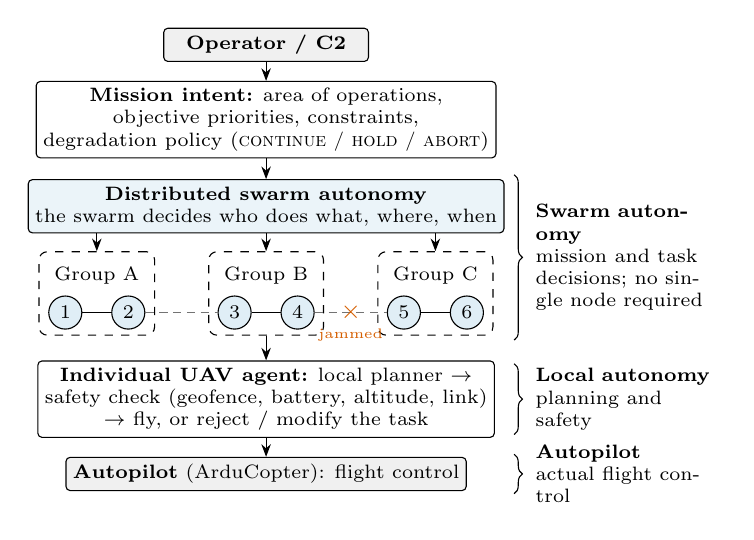
\begin{tikzpicture}[font=\scriptsize, >={Stealth[length=1.6mm]},
  blk/.style={draw, rounded corners=1.5pt, align=center, inner sep=2.5pt, fill=white},
  uav/.style={circle, draw, fill=cDist!12, inner sep=0pt, minimum size=4.2mm},
  grp/.style={draw, dashed, rounded corners=3pt, inner sep=2pt},
  tier/.style={align=left, anchor=west, text width=2.3cm}]
  % ---- vertical stack ------------------------------------------------------
  \node[blk, fill=black!6, minimum width=2.6cm] (op) at (2.9,0)
    {\textbf{Operator / C2}};
  \node[blk, minimum width=5.6cm] (intent) at (2.9,-0.95)
    {\textbf{Mission intent:} area of operations,\\ objective priorities, constraints,\\
     degradation policy (\textsc{continue / hold / abort})};
  \node[blk, fill=cDist!8, minimum width=5.8cm] (dsa) at (2.9,-2.05)
    {\textbf{Distributed swarm autonomy}\\ the swarm decides who does what, where, when};
  % groups
  \node (la) at (0.75,-2.93) {Group A};
  \node (lb) at (2.90,-2.93) {Group B};
  \node (lc) at (5.05,-2.93) {Group C};
  \node[uav] (a1) at (0.35,-3.4) {1};
  \node[uav] (a2) at (1.15,-3.4) {2};
  \node[uav] (b1) at (2.50,-3.4) {3};
  \node[uav] (b2) at (3.30,-3.4) {4};
  \node[uav] (c1) at (4.65,-3.4) {5};
  \node[uav] (c2) at (5.45,-3.4) {6};
  \node[grp, fit=(la)(a1)(a2)] (gA) {};
  \node[grp, fit=(lb)(b1)(b2)] (gB) {};
  \node[grp, fit=(lc)(c1)(c2)] (gC) {};
  \draw (a1) -- (a2);  \draw (b1) -- (b2);  \draw (c1) -- (c2);
  \draw[densely dashed, black!55] (a2) -- (b1);
  \draw[densely dashed, black!55] (b2) -- (c1);
  \node[text=cCent, font=\bfseries\small] at ($(b2)!0.5!(c1)$) {$\times$};
  \node[text=cCent, font=\tiny] at ($(b2)!0.5!(c1)+(0,-0.28)$) {jammed};
  \foreach \g in {gA,gB,gC} \draw[->] (dsa.south -| \g.north) -- (\g.north);
  % individual UAV and autopilot
  \node[blk, minimum width=4.6cm] (agent) at (2.9,-4.5)
    {\textbf{Individual UAV agent:} local planner $\rightarrow$\\
     safety check (geofence, battery, altitude, link)\\
     $\rightarrow$ fly, or reject / modify the task};
  \node[blk, fill=black!6, minimum width=3.6cm] (ap) at (2.9,-5.45)
    {\textbf{Autopilot} (ArduCopter): flight control};
  \draw[->] (gB.south) -- (agent.north);
  \draw[->] (agent.south) -- (ap.north);
  \draw[->] (op.south) -- (intent.north);
  \draw[->] (intent.south) -- (dsa.north);
  % ---- responsibility tiers -------------------------------------------------
  \draw[decorate, decoration={brace, amplitude=3pt}] (6.05,-1.65) -- (6.05,-3.75);
  \node[tier] at (6.2,-2.7) {\textbf{Swarm autonomy}\\ mission and task decisions; no single node required};
  \draw[decorate, decoration={brace, amplitude=3pt}] (6.05,-4.05) -- (6.05,-4.95);
  \node[tier] at (6.2,-4.5) {\textbf{Local autonomy}\\ planning and safety};
  \draw[decorate, decoration={brace, amplitude=3pt}] (6.05,-5.2) -- (6.05,-5.7);
  \node[tier] at (6.2,-5.45) {\textbf{Autopilot}\\ actual flight control};
\end{tikzpicture}}
\caption{Concept of operations, redrawn from the team's design notebook
(Appendix~\ref{app:sketches}). The operator supplies intent, not a plan.
Groups that lose contact (the jammed link) continue from local knowledge and
synchronise when contact returns. Each UAV can reject a swarm task that fails
its local safety check.}
\label{fig:conops}
\end{figure}

% =============================================================================
\section{Related Work}
\label{sec:related}

\emph{Multi-robot task allocation.} Allocation taxonomies~\cite{gerkey2004taxonomy}
and auction/consensus methods such as CBBA~\cite{choi2009cbba} reach
conflict-free assignments when bids eventually propagate. Recent
communication-aware allocators combine topology construction with robust
auction-consensus and report resilience to packet loss, delay and topology
switching in simulation~\cite{lu2026commaware}. Communication-aware
allocation is therefore not new. Our target is different: what a UAV may
\emph{execute} while bids cannot propagate at all, and how replicas converge
afterwards, without importing a globally coherent bid view.

\emph{Partition-tolerant replicated state.} Surveys of UAV networking
describe intermittent links and rapidly changing topologies as the norm in
flying ad-hoc networks~\cite{bekmezci2013fanet,hayat2016survey}.
Availability-first replication
with eventual convergence is well established in distributed
systems~\cite{decandia2007dynamo,vogels2009eventually,shapiro2011crdt},
built on epidemic dissemination~\cite{demers1987epidemic}. Leases bound the
validity of cached authority without synchronous revocation~\cite{gray1989leases}.
In swarm robotics, SwarmDAG lets disconnected groups continue recording
progress and later merge toward eventual consistency~\cite{tran2019swarmdag},
and the CHARISMA project describes a distributed shared-memory service for
heterogeneous unmanned vehicles~\cite{charisma}. Partition tolerance by itself
is thus prior art. We claim no novelty for it. Our contribution is in the
receiver-local semantics of ownership, evidence and execution authority, and
in measuring what they buy.

\emph{Failure detection and consensus.} Consensus-based reassignment, \eg
Paxos~\cite{lamport1998paxos} or Raft~\cite{ongaro2014raft}, needs a majority
that can communicate. Unreliable failure detectors~\cite{chandra1996unreliable}
formalise why silence is ambiguous. We keep a quorum-certified declaration,
but we deliberately decouple task recovery from it.

\emph{Formal discrete control.} Supervisory control theory has been applied
to robot swarms with up to 600 physical robots~\cite{lopes2016sct};
statechart-based mission execution separates UAS mission logic from flight
control~\cite{santamaria2010mission}; automata-based frameworks synthesise
multi-agent plans from capability models~\cite{tziola2026formal}. Industrial
interfaces also expose explicit, versioned task lifecycles with terminal
states~\cite{anduril_lattice}. Following this line, we keep finite-state
structure around discrete decisions and leave radio, geometry and
optimisation numerical.

\emph{Search and coverage.} Boustrophedon
decomposition~\cite{choset2000boustrophedon,galceran2013coverage}, communication-constrained coverage~\cite{loizou2016dendritic},
and distributed receding-horizon 3-D search with a varying number of
agents~\cite{papaioannou2023glimpse} address \emph{how} an area is searched.
We use the simplest of these (sector strips with boustrophedon lanes) only to
exercise \emph{who} may search each sector. CARIC~\cite{cao2025caric} is a
candidate external benchmark for future comparisons.

\emph{Quantum optimisation.} QAOA~\cite{farhi2014qaoa} and the quantum
alternating operator ansatz with constraint-preserving XY
mixers~\cite{hadfield2019qaoa,wang2020xy} apply to QUBO-encoded assignment
problems~\cite{lucas2014ising}. Practical advantage remains problem- and
hardware-dependent~\cite{blekos2024qaoa}, and simulated QAOA has been proposed
for network subproblems~\cite{chen2025distributedqc}. We use QAOA only as an
advisory planner and report it against classical and random baselines.

% =============================================================================
\section{System Model and Design Rule}
\label{sec:model}

\emph{Agents and tasks.} A swarm has $N$ UAVs with distinct, totally ordered
identifiers $V=\{1,\dots,N\}$. The mission is an immutable catalogue
$\mathcal{J}$ of objectives (identifier and position) handed to every UAV at
start. In the live mission (Section~\ref{sec:live}), new objectives are
discovered from geolocated detections. Mutable task records exist only as an
observer-facing projection and are never an input to control.

\emph{Communication.} The world model maintains a time-varying undirected
graph $G(t)=(V,E(t))$. In the simulator an edge exists if both endpoints are
within a communication range $R$, the link is not explicitly blocked, and no
active region jammer covers the link's midpoint. An optional free-space
line-of-sight link model with seeded stochastic delivery also exists, but it
is an analytical abstraction, not calibrated RF. Messages travel hop by hop
over $E(t)$ only. Network conditions range from connected, through degraded
and partitioned, to an isolated UAV; we treat all of them as normal operating
modes.

\emph{Faults and clocks.} UAVs fail by stopping (fail-stop): a failed UAV
neither moves, transmits, relays nor renews. We do not model Byzantine
behaviour or identity forgery. Each UAV measures ages on its own clock from
the moment it first accepted a piece of evidence. Source timestamps are
metadata and are never compared with the receiver's clock to make a decision.
The simulator happens to drive every replica from one deterministic logical
clock, but decision logic does not rely on that, and no decision orders events
across UAVs by their clocks~\cite{lamport1978time}.

\begin{definition}[Receiver-local knowledge and the epistemic rule]
Let $K_i(t)$ be UAV~$i$'s own state together with every evidence item
delivered to $i$ up to time $t$, each stamped with its local receipt time. A
control transition of $i$ at time $t$ is \emph{admissible} only if its guard
is a function of $K_i(t)$, $t$ and $i$ alone.
\end{definition}

The rule excludes, in particular, graph reachability (a radio cannot report
that a link is down; only silence accumulates), another UAV's live position or
task, mission-wide failure projections, and anything computed by the
evaluator. Table~\ref{tab:layers} lists the three kinds of state that coexist
in one process and the direction in which information may flow between them.
Architecture tests fail the build if, for example, the autonomy module imports
the simulator or the dashboard imports authoritative world state.

\begin{table}[t]
\caption{Three kinds of state and what each must not do}
\label{tab:layers}
\centering
\footnotesize
\begin{tabular}{@{}L{1.35cm}L{3.3cm}L{3.15cm}@{}}
\toprule
Layer & Holds & Must not \\
\midrule
World / physics &
true positions and responsiveness, $G(t)$, radio and jammer models, observer
task projection &
supply remote state or graph truth to decisions; authorise ownership \\
Receiver-local control &
own state, task catalogue, local utility, peer-state store, claim ledger,
EFSM kernel, held contract &
infer failure from silence alone; act without local ownership \\
Observer / evaluation &
metrics, traces, dashboard, operator map, test assertions &
feed its privileged view back into any decision \\
\bottomrule
\end{tabular}
\end{table}

\emph{Design goals.} (G1)~\emph{Availability under partition:} every
connected group keeps working on unowned objectives. (G2)~\emph{Convergence:}
after connectivity is stably restored, every task has one owner at every
replica. (G3)~\emph{No single required node} in the protocol, including a
coordinator or a ground station on the coordination path (the live harness of
Section~\ref{sec:live} still co-locates all agents on one ground node; see
Section~\ref{sec:discussion}). (G4)~\emph{Operator restraint:} the
operator chooses how much risk of duplicated work the mission accepts.
(G5)~\emph{Human authority over engagement} in the live mission.
Fig.~\ref{fig:arch} shows how the components of each UAV's agent, as first
sketched in the design notebook, map onto the three layers and onto the
implementation.

% -----------------------------------------------------------------------------
\begin{figure*}[t]
\centering
\resizebox{\textwidth}{!}{%
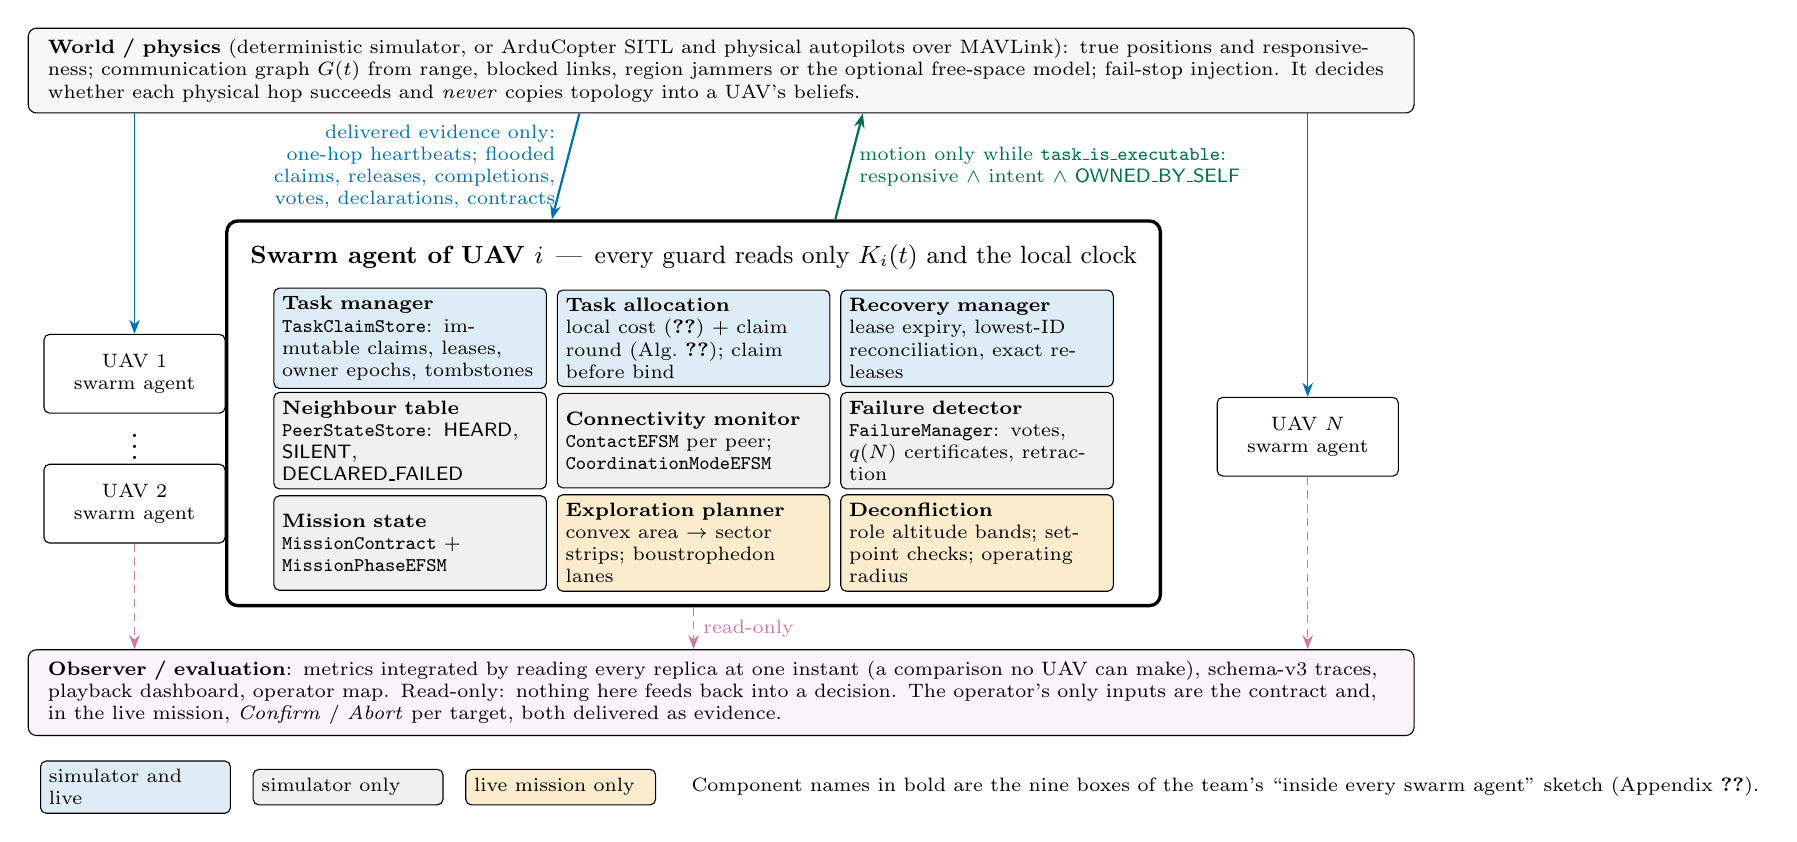
\begin{tikzpicture}[font=\scriptsize, >={Stealth[length=1.8mm]},
  band/.style={draw, rounded corners=3pt, minimum width=17.6cm, align=left,
               inner sep=4pt, text width=17.1cm},
  cell/.style={draw, rounded corners=2pt, text width=3.25cm, minimum height=1.2cm,
               align=left, inner sep=3pt, font=\scriptsize},
  both/.style={cell, fill=cDist!13},
  sim/.style={cell, fill=black!6},
  live/.style={cell, fill=cOrange!20},
  small/.style={draw, rounded corners=2pt, align=center, minimum width=2.3cm,
                minimum height=1.0cm, fill=white}]
  % world band
  \node[band, fill=black!3] (world) at (8.8,1.55)
    {\textbf{World / physics} (deterministic simulator, or ArduCopter SITL and
     physical autopilots over MAVLink): true positions and responsiveness;
     communication graph $G(t)$ from range, blocked links, region jammers or the
     optional free-space model; fail-stop injection. It decides whether each
     physical hop succeeds and \emph{never} copies topology into a UAV's beliefs.};
  % agent grid
  \node[both] (c11) at (4.85,-1.85) {\textbf{Task manager}\\ \code{TaskClaimStore}: immutable claims, leases, owner epochs, tombstones};
  \node[both] (c12) at (8.45,-1.85) {\textbf{Task allocation}\\ local cost~\eqref{eq:cost} + claim round (Alg.~\ref{alg:round}); claim before bind};
  \node[both] (c13) at (12.05,-1.85) {\textbf{Recovery manager}\\ lease expiry, lowest-ID reconciliation, exact releases};
  \node[sim]  (c21) at (4.85,-3.15) {\textbf{Neighbour table}\\ \code{PeerStateStore}: \stt{HEARD}, \stt{SILENT},\\ \stt{DECLARED\_FAILED}};
  \node[sim]  (c22) at (8.45,-3.15) {\textbf{Connectivity monitor}\\ \code{ContactEFSM} per peer; \code{CoordinationModeEFSM}};
  \node[sim]  (c23) at (12.05,-3.15) {\textbf{Failure detector}\\ \code{FailureManager}: votes, $q(N)$ certificates, retraction};
  \node[sim]  (c31) at (4.85,-4.45) {\textbf{Mission state}\\ \code{MissionContract} + \code{MissionPhaseEFSM}};
  \node[live] (c32) at (8.45,-4.45) {\textbf{Exploration planner}\\ convex area $\rightarrow$ sector strips; boustrophedon lanes};
  \node[live] (c33) at (12.05,-4.45) {\textbf{Deconfliction}\\ role altitude bands; setpoint checks; operating radius};
  \node[font=\small, anchor=south] (atitle) at (8.45,-1.1)
    {\textbf{Swarm agent of UAV $i$} \,---\, every guard reads only $K_i(t)$ and the local clock};
  \node[draw, very thick, rounded corners=4pt, inner sep=5pt, fit=(atitle)(c11)(c33)] (agent) {};
  % other agents
  \node[small] (u1) at (1.35,-2.3) {UAV $1$\\ swarm agent};
  \node[small] (u2) at (1.35,-3.95) {UAV $2$\\ swarm agent};
  \node[small] (un) at (16.25,-3.1) {UAV $N$\\ swarm agent};
  \node[font=\large] at (1.35,-3.12) {$\vdots$};
  % observer band
  \node[band, fill=cPurple!8] (obs) at (8.8,-6.35)
    {\textbf{Observer / evaluation}: metrics integrated by reading every replica
     at one instant (a comparison no UAV can make), schema-v3 traces, playback
     dashboard, operator map. Read-only: nothing here feeds back into a decision.
     The operator's only inputs are the contract and, in the live mission,
     \emph{Confirm} / \emph{Abort} per target, both delivered as evidence.};
  % arrows world <-> agents
  \draw[->, thick, cDist] ($(world.south)+(-1.8,0)$) -- node[left, align=right, font=\scriptsize]
    {delivered evidence only:\\ one-hop heartbeats; flooded\\ claims, releases, completions,\\
     votes, declarations, contracts} ($(agent.north)+(-1.8,0)$);
  \draw[<-, thick, cGreen!70!black] ($(world.south)+(1.8,0)$) -- node[right, align=left, font=\scriptsize]
    {motion only while \code{task\_is\_executable}:\\ responsive $\wedge$ intent $\wedge$ \stt{OWNED\_BY\_SELF}} ($(agent.north)+(1.8,0)$);
  \draw[->, densely dashed, cPurple] (agent.south) -- node[right, font=\scriptsize] {read-only} (obs.north -| agent.south);
  \draw[->, densely dashed, cPurple] (u2.south) -- (u2.south |- obs.north);
  \draw[->, densely dashed, cPurple] (un.south) -- (un.south |- obs.north);
  \draw[->, cDist] (u1.north |- world.south) -- (u1.north);
  \draw[->, cDist] (un.north |- world.south) -- (un.north);
  % legend
  \node[both, text width=2.2cm, minimum height=0.45cm, anchor=west] (k1) at (0.15,-7.55) {simulator and live};
  \node[sim,  text width=2.2cm, minimum height=0.45cm, anchor=west] (k2) at (2.85,-7.55) {simulator only};
  \node[live, text width=2.2cm, minimum height=0.45cm, anchor=west] (k3) at (5.55,-7.55) {live mission only};
  \node[anchor=west, font=\scriptsize] at (8.3,-7.55)
    {Component names in bold are the nine boxes of the team's ``inside every swarm agent'' sketch (Appendix~\ref{app:sketches}).};
\end{tikzpicture}}
\caption{Architecture. The world layer gates every physical hop but never
supplies beliefs; each UAV's agent decides only from delivered evidence; the
observer layer reads everything and writes nothing. Shading shows where each
sketched component is implemented today.}
\label{fig:arch}
\end{figure*}

% =============================================================================
\section{Receiver-Local Coordination Protocol}
\label{sec:protocol}

\subsection{Evidence and dissemination}
\label{sec:evidence}

Two kinds of message exist. \emph{Heartbeats} are one-hop by design: receiving
one means first-hand contact with its source. Everything else is
\emph{immutable protocol evidence}: task claims, releases, completions,
failure votes, failure declarations and mission-contract versions. Immutable
evidence is flooded deterministically over the current connected component
(store-and-forward). Each item has a content-derived structural identity, \eg
$(j,o,e)$ for a claim. Every receiver applies an item at most once, forwards
it to neighbours in sorted order, and retains failed directed routes for retry
when the topology changes. Finite membership and per-node seen-state make
flooding terminate without a time-to-live. Forwarding metadata (logical
origin, forwarder, receiver, hop count) lives in the transport envelope; a
relay never becomes the author of what it carries. A duplicate delivery never
refreshes the age of evidence it repeats.

\subsection{Peer status and quorum-certified failure}
\label{sec:failure}

Each UAV keeps a peer-state store that derives, for every peer, one of three
statuses (\stt{HEARD}, \stt{SILENT} or \stt{DECLARED\_FAILED}) from
delivered heartbeats and elapsed local time. There is no status meaning ``the link is
down''. A UAV may create a \emph{failure vote} for a peer only after hearing
nothing for strictly longer than the heartbeat timeout. It may create a
\emph{declaration} only when its own mailbox holds enough fresh, matching
votes, its own among them. The threshold is
\begin{equation}
  q(N) \;=\; \max\!\Bigl(2,\; \bigl\lfloor (N-1)/2 \bigr\rfloor + 1\Bigr).
  \label{eq:quorum}
\end{equation}

\begin{proposition}[No unilateral declaration]
\label{prop:floor}
For every $N$, $q(N)\ge 2$: no UAV can certify a peer's failure from its own
evidence alone. For $N=2$ no failure can ever be declared.
\end{proposition}
\begin{IEEEproof}
Immediate from~\eqref{eq:quorum}; for $N=2$ the only possible voter is the
single survivor, and $1<q(2)=2$.
\end{IEEEproof}

\begin{proposition}[Quorum intersection]
\label{prop:intersection}
For any suspect $s$ and $N\ge 3$, any two voter sets that each reach $q(N)$
intersect. Two groups that exchange no votes therefore cannot both certify
$s$ from votes created within each group.
\end{proposition}
\begin{IEEEproof}
Voters are drawn from $V\setminus\{s\}$, which has $N-1$ members. For $N\ge3$,
$q(N)=\lfloor (N-1)/2\rfloor+1>(N-1)/2$, so two disjoint qualifying sets
would need more than $N-1$ members.
\end{IEEEproof}

A certificate is \emph{corroborated belief, not proof}: there is no positive
remote-health signal, so a quorum can wrongly declare a healthy UAV that sits
behind a partition. Declarations are therefore reversible: a newly delivered
heartbeat from the declared peer outranks a second-hand certificate and
retracts it. A declaration never stops a vehicle. A wrongly declared UAV keeps
flying and keeps the task it does not know it lost; ownership reconciliation,
not the detector, repairs that.

\subsection{Lease-based task ownership}
\label{sec:leases}

Each UAV keeps an independent claim ledger (\code{TaskClaimStore}). A claim
$c=(j,o,e)$ states that owner $o$ claims task $j$ at owner-scoped epoch $e$;
it is an immutable value. Receiver $i$ records the time $\rho_i(c)$ at which
it first accepted $c$ and computes the age $a_i(c,t)=t-\rho_i(c)$. With a
freshness threshold $F$ and a lease duration $L$, $0<F<L$, the claim is
\begin{equation}
  \text{fresh if } a\le F,\quad
  \text{stale if } F<a\le L,\quad
  \text{expired if } a>L .
  \label{eq:lease}
\end{equation}
\emph{Stale is not free}: a stale claim is still lease-valid, and a UAV may
create a competing claim only when every incompatible claim it knows is
expired or explicitly released. An owner renews by issuing the next epoch
when its own copy reaches age $F$ (default $F=L/2$), not on every tick.
Epochs are compared only within one $(j,o)$ stream: a higher epoch supersedes
lower ones from the same owner, a delayed lower epoch is ignored, the same
$(j,o,e)$ with a different payload is rejected as contradictory, and a release
tombstone prevents a delayed copy from resurrecting ownership. Epochs from
different owners are never compared.

From its ledger, receiver $i$ derives a six-state interpretation $S_{ij}(t)$
of task $j$ (Fig.~\ref{fig:ownership}). The vocabulary is deliberately exact.
\stt{UNCLAIMED} means ``$i$ has no lease-valid claim evidence for $j$'', not
``nobody owns $j$''. Two partitioned UAVs may both report
\stt{OWNED\_BY\_SELF}; this split-brain state is allowed and represented, not
a bug.

\begin{figure}[t]
\centering
\resizebox{\columnwidth}{!}{%
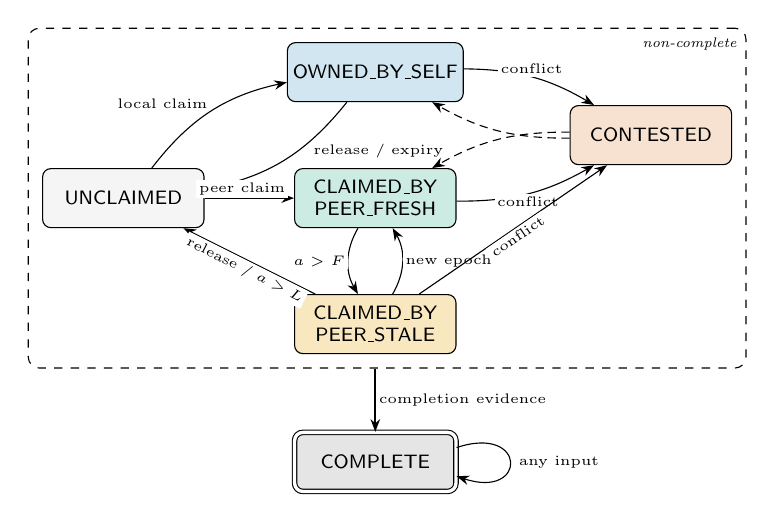
\begin{tikzpicture}[font=\scriptsize, >={Stealth[length=1.6mm]},
  st/.style={draw, rounded corners=3pt, align=center, minimum width=2.05cm,
             minimum height=0.75cm, inner sep=2pt, font=\scriptsize\sffamily},
  lab/.style={font=\tiny, inner sep=1pt, fill=white}]
  \node[st, fill=black!4]      (U) at (0,2.0)   {UNCLAIMED};
  \node[st, fill=cDist!18]     (O) at (3.2,3.6) {OWNED\_BY\_SELF};
  \node[st, fill=cGreen!20]    (F) at (3.2,2.0) {CLAIMED\_BY\\PEER\_FRESH};
  \node[st, fill=cOrange!25]   (S) at (3.2,0.4) {CLAIMED\_BY\\PEER\_STALE};
  \node[st, fill=cCent!18]     (C) at (6.7,2.8) {CONTESTED};
  \node[st, double, double distance=1.2pt, fill=black!10] (D) at (3.2,-1.35) {COMPLETE};
  % U <-> O
  \draw[->] (U) to[bend left=20] node[lab, above left] {local claim} (O);
  \draw[->] (O) to[bend left=20] node[lab, below right, pos=0.3] {release / expiry} (U);
  % U -> F, S -> U
  \draw[->] (U) -- node[lab, above, pos=0.42] {peer claim} (F);
  \draw[->] (S) -- node[lab, below, sloped] {release / $a>L$} (U);
  % F <-> S
  \draw[->] (F) to[bend right=30] node[lab, left] {$a>F$} (S);
  \draw[->] (S) to[bend right=30] node[lab, right] {new epoch} (F);
  % conflicts (solid) and reconciliation outcomes (dashed)
  \draw[->] (O) to[bend left=15] node[lab, above] {conflict} (C);
  \draw[->, densely dashed] (C) to[bend left=15] (O);
  \draw[->] (F) to[bend right=15] node[lab, below] {conflict} (C);
  \draw[->, densely dashed] (C) to[bend right=15] (F);
  \draw[->] (S) -- node[lab, below, sloped] {conflict} (C);
  % completion
  \node[draw, dashed, rounded corners=4pt, inner sep=5pt, fit=(U)(O)(S)(C)] (NC) {};
  \node[font=\tiny\itshape, anchor=north east] at (NC.north east) {non-complete};
  \draw[->, thick] (NC.south -| D.north) -- node[lab, right] {completion evidence} (D.north);
  \draw[->] (D.10) .. controls +(0.9,0.3) and +(0.9,-0.3) .. (D.-10);
  \node[lab, anchor=west] at ($(D.east)+(0.75,0)$) {any input};
\end{tikzpicture}}
\caption{Receiver-local task-ownership interpretation $S_{ij}$ (one machine
per task per UAV). ``Conflict'' means an incompatible lease-valid claim
becomes visible; dashed arrows are reconciliation outcomes (self or peer;
selecting a stale peer is also possible, edge omitted). \stt{COMPLETE} is
absorbing.}
\label{fig:ownership}
\end{figure}

\subsection{Deterministic reconciliation and completion}
\label{sec:reconcile}

When more than one owner's latest claim is lease-valid at receiver $i$, then
$S_{ij}=\stt{CONTESTED}$. Freshness does not break the tie: a stale but
lease-valid claim is a real contender. Conflict handling has three explicit
phases. \emph{Observe}: the receiver keeps every contender and reports
\stt{CONTESTED}. \emph{Reconcile}: it selects the claim with the lowest owner
identifier,
\begin{equation}
  w_{ij}(t) \;=\; \min\,\{\, o \;:\; (j,o,\cdot)\in \mathcal{C}_{ij}(t) \,\},
  \label{eq:winner}
\end{equation}
where $\mathcal{C}_{ij}(t)$ is the set of latest lease-valid, unreleased
per-owner claims known to $i$. \emph{Release}: if $i$ itself lost, it stops
acting as owner immediately and floods an exact-generation release that
names the winning claim. Completion evidence can be created only by the
current lease-valid owner and carries the claim it completes. Once accepted,
it makes $S_{ij}=\stt{COMPLETE}$ permanently, whatever arrives later.

\begin{proposition}[Agreement and post-partition convergence]
\label{prop:converge}
(a) Any two receivers with the same set of owners in $\mathcal{C}_{ij}$ select
the same winner, independently of message order. (b) Suppose that from time
$t_h$ the responsive UAVs form a connected component of $G(t)$ that remains
stable, that each claimant keeps renewing while it believes it owns $j$, and
that no new conflicting claim is created. Then within the time needed to flood
the renewals and the losers' releases, every replica in the component holds
the single owner $w=\min$ of the claimants.
\end{proposition}
\begin{IEEEproof}[Proof sketch]
(a) Equation~\eqref{eq:winner} is a function of the owner set over a total
order. (b) Flooding delivers every immutable item to every node of a stable
connected component in at most its diameter of rounds. Each claimant renews
at age $F<L$, so once renewals are delivered all replicas hold every
claimant's latest claim as lease-valid and agree on $w$ by (a). Each loser
$\ell$ holds the same set, so it releases. Its release floods, and tombstones
remove $\ell$'s generation everywhere. Thereafter $\ell$ sees $j$ as
\stt{CLAIMED\_BY\_PEER\_*} and cannot re-claim while $w$ renews.
\end{IEEEproof}
Proposition~\ref{prop:converge} is argued, not machine-checked. It is
exercised by deterministic integration tests, including split-brain
reconciliation through the four-node chain $1\!-\!2\!-\!3\!-\!4$. Note that
the lowest-identifier rule is a correctness mechanism that makes replicas
agree, not a utility-optimal allocator.

\subsection{Recovery without declaration}
\label{sec:recovery}

\begin{proposition}[Declaration-free recovery bound]
\label{prop:recovery}
Let owner $o$ of task $j$ fail-stop at time $t_f$, and let receiver $r$
accept $o$'s last claim generation at time $\rho_r$. If $r$ knows of no other
valid claim on $j$, then $j$ is claimable at $r$ for every $t>\rho_r+L$,
whether or not any failure declaration about $o$ exists. If that generation
was created at or before $t_f$ and reached $r$ after a dissemination delay of
at most $\delta$, the task is claimable at $r$ after
$t_f+\delta+L$.
\end{proposition}
\begin{IEEEproof}
A fail-stopped owner creates no new epoch. By~\eqref{eq:lease} the copy at $r$
expires once $a_r>L$, and no guard on the claim path reads peer status. The
second statement follows from $\rho_r\le t_f+\delta$.
\end{IEEEproof}

A coordinator that reassigns only on a declaration has no such bound. The
declaration requires $q(N)$ responsive voters, connected to one another and to
the coordinator. If that never happens, as with $N=2$ (Proposition~\ref{prop:floor})
or a sparse or jammed graph, the task is held by a stopped aircraft
indefinitely.
Fig.~\ref{fig:lease} contrasts the two paths. Activation additionally needs an
idle UAV, so the bound is on \emph{availability}, not on completion.

\begin{figure}[t]
\centering
\resizebox{\columnwidth}{!}{%
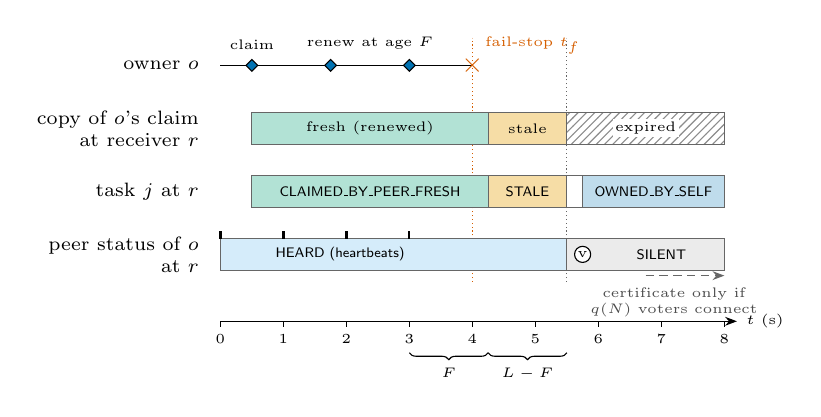
\begin{tikzpicture}[font=\scriptsize, >={Stealth[length=1.5mm]},
  lane/.style={anchor=east, align=right, font=\scriptsize}]
  % lane labels (outside the time scope)
  \node[lane] at (1.85,2.4) {owner $o$};
  \node[lane] at (1.85,1.6) {copy of $o$'s claim\\ at receiver $r$};
  \node[lane] at (1.85,0.8) {task $j$ at $r$};
  \node[lane] at (1.85,0.0) {peer status of $o$\\ at $r$};
  \begin{scope}[xshift=2.0cm, x=0.8cm, y=1cm]
    % reference lines
    \draw[densely dotted, cCent] (4,-0.35) -- (4,2.75);
    \draw[densely dotted, black!60] (5.5,-0.35) -- (5.5,2.75);
    % owner lane
    \draw (0,2.4) -- (4,2.4);
    \foreach \x in {0.5,1.75,3.0}
      \node[diamond, draw, fill=cDist, inner sep=1.1pt] at (\x,2.4) {};
    \node[font=\tiny, above] at (0.5,2.48) {claim};
    \node[font=\tiny, above] at (2.375,2.48) {renew at age $F$};
    \node[text=cCent, font=\bfseries] at (4,2.4) {$\times$};
    \node[font=\tiny, text=cCent, above right] at (4.05,2.42) {fail-stop $t_f$};
    % claim copy lane
    \filldraw[fill=cGreen!30, draw=black!60] (0.5,1.4) rectangle (4.25,1.8);
    \filldraw[fill=cOrange!35, draw=black!60] (4.25,1.4) rectangle (5.5,1.8);
    \filldraw[pattern=north east lines, pattern color=black!45, draw=black!60] (5.5,1.4) rectangle (8,1.8);
    \node[font=\tiny] at (2.375,1.6) {fresh (renewed)};
    \node[font=\tiny] at (4.875,1.6) {stale};
    \node[font=\tiny, fill=white, inner sep=1pt] at (6.75,1.6) {expired};
    % task lane
    \filldraw[fill=cGreen!30, draw=black!60] (0.5,0.6) rectangle (4.25,1.0);
    \filldraw[fill=cOrange!35, draw=black!60] (4.25,0.6) rectangle (5.5,1.0);
    \filldraw[fill=white, draw=black!60] (5.5,0.6) rectangle (5.75,1.0);
    \filldraw[fill=cDist!25, draw=black!60] (5.75,0.6) rectangle (8,1.0);
    \node[font=\tiny\sffamily] at (2.375,0.8) {CLAIMED\_BY\_PEER\_FRESH};
    \node[font=\tiny\sffamily] at (4.875,0.8) {STALE};
    \node[font=\tiny\sffamily] at (6.875,0.8) {OWNED\_BY\_SELF};
    % peer-status lane
    \filldraw[fill=cSky!25, draw=black!60] (0,-0.2) rectangle (5.5,0.2);
    \filldraw[fill=black!8, draw=black!60] (5.5,-0.2) rectangle (8,0.2);
    \foreach \x in {0,1,2,3} \draw[thick] (\x,0.2) -- (\x,0.3);
    \node[font=\tiny\sffamily] at (1.9,0) {HEARD (heartbeats)};
    \node[font=\tiny\sffamily] at (7.0,0) {SILENT};
    \node[draw, circle, inner sep=0.6pt, font=\tiny, fill=white] (v) at (5.75,0) {v};
    \draw[->, densely dashed, black!60] (6.75,-0.27) -- (8,-0.27);
    \node[font=\tiny, below, align=center, black!70] at (7.2,-0.3)
      {certificate only if\\ $q(N)$ voters connect};
    % time axis
    \draw[->] (0,-0.85) -- (8.2,-0.85) node[right, font=\tiny] {$t$ (s)};
    \foreach \x in {0,...,8} {
      \draw (\x,-0.85) -- (\x,-0.92);
      \node[font=\tiny, below] at (\x,-0.9) {\x};
    }
    % braces
    \draw[decorate, decoration={brace, mirror, amplitude=2.5pt}]
      (3.0,-1.25) -- node[below=2pt, font=\tiny] {$F$} (4.25,-1.25);
    \draw[decorate, decoration={brace, mirror, amplitude=2.5pt}]
      (4.25,-1.25) -- node[below=2pt, font=\tiny] {$L-F$} (5.5,-1.25);
  \end{scope}
\end{tikzpicture}}
\caption{Recovery from a fail-stop with the default $L=2.5$\,s, $F=L/2$,
heartbeat interval 1\,s and silence timeout 2.5\,s. The task becomes
claimable at $r$ when its copy of the last renewal expires
(Proposition~\ref{prop:recovery}). The failure vote ``v'' and any certificate
are not on this path; a certificate may never form.}
\label{fig:lease}
\end{figure}

\subsection{Receiver-local task selection}
\label{sec:utility}

Each idle UAV ranks the objectives it can claim, $A_i(t)$ (not complete at
$i$, with every known incompatible claim expired or released), by an additive
cost evaluated only from its own state and delivered evidence:
\begin{equation}
  \mathrm{cost}_i(j)=w_{\mathrm{d}}\lVert p_i-p_j\rVert
  + w_{\mathrm{r}}\,r_i(j) + w_{\mathrm{c}}\,\kappa_i(j) + w_{\mathrm{o}}\,\varrho_i(j),
  \label{eq:cost}
\end{equation}
with ties broken by task identifier. Here $r_i$ and $\varrho_i$ are resource
and role terms, and $\kappa_i(j)=(N-1)-\hat d_i(p_j)$ is a
communication term: $\hat d_i$ counts peers whose \emph{last delivered,
still \stt{HEARD}} position lies within range of $p_j$. The term never reads
$G(t)$. By default only distance is weighted. The original design note asked
for a richer utility (information gain minus travel, energy, communication
and operational risk), on the observation that ``the closest UAV is not always
the best UAV''; Eq.~\eqref{eq:cost} implements the travel and communication
parts and keeps resource and role as validated extension points. The live
mission expresses one role preference, holding physical vehicles in reserve,
as a receiver-local delay rule (Section~\ref{sec:engage}).

Algorithm~\ref{alg:round} is the task-control round run at every event
boundary. Choices are batched from pre-mutation views, so agent traversal
order cannot silently allocate a task. A claim exists before an intent is
bound, and a single predicate, \code{task\_is\_executable}, gates motion,
renewal and completion. It requires that the UAV is responsive, that its
cached intent names the task, and that its own ledger reports
\stt{OWNED\_BY\_SELF}.

\begin{algorithm}[t]
\caption{Receiver-local task-control round at time $t$}
\label{alg:round}
\begin{algorithmic}[1]
\For{each participating UAV $i$}
  \State advance the lease clock of ledger $i$ to $t$
  \State stand down unless ledger $i$ still owns intent $j_i$
  \If{$j_i\neq\bot$ \textbf{and} $a_i(c_i,t)\ge F$}
    \State renew: create $(j_i,i,e+1)$
  \EndIf
\EndFor
\Repeat
  \State $P\gets\{(i,\arg\min_{j\in A_i(t)}\mathrm{cost}_i(j)) : i \text{ idle}\}$
  \State create a claim $(j,i,e_{ij}+1)$ for every $(i,j)\in P$
  \State flood new immutable evidence over $G(t)$
  \State each $i$ reconciles contests; losers release
  \State each idle $i$ owning its claim binds intent $j_i\gets j$
\Until{no claim, stand-down or activation occurred}
\end{algorithmic}
\end{algorithm}

\subsection{Composed EFSM kernel and the mission contract}
\label{sec:efsm}

Each UAV composes small machines instead of one product automaton
(Table~\ref{tab:efsm}). Every transition is a pure function
\begin{equation*}
  \delta\bigl((q,x),e,\pi\bigr)\mapsto(q',x',\mathcal{E},g,\mathit{reason}),
\end{equation*}
of finite state $q$, typed extended variables $x$, a typed local event $e$ and
a policy $\pi$. It returns the next configuration, a list of requested effects
$\mathcal{E}$ and the guard $g$ and reason that justified it. Reducers never
move a vehicle, send a packet or read observer state. Effects are data, and
in the current prototype the coordination mode is advisory: execution
authority remains the claim ledger. Contact recovery requires receipts at
\emph{distinct} local times, so a same-timestamp burst cannot manufacture
stability. Contact evidence is attributed to the immediate forwarder, not to
a message's logical origin.

\begin{table}[t]
\caption{Composed receiver-local EFSMs (per UAV)}
\label{tab:efsm}
\centering
\footnotesize
\begin{tabular}{@{}L{1.25cm}L{0.7cm}L{2.75cm}L{2.7cm}@{}}
\toprule
Machine & Count & States & Driven by \\
\midrule
Contact & per peer &
\stt{UNKNOWN}, \stt{ACTIVE}, \stt{DEGRADED}, \stt{LOST}, \stt{RECOVERING} &
direct-hop receipts; local time \\
Peer avail. & per peer &
\stt{SILENT}, \stt{HEARD}, \stt{DECLARED\_FAILED} &
first-hand heartbeat; silence; valid certificate \\
Task owner. & per task & six states of Fig.~\ref{fig:ownership} &
local ledger view (conformance) \\
Coordin. mode & one &
\stt{COOPERATIVE}, \stt{DEGRADED}, \stt{LOCAL\_AUTONOMY}, \stt{RECONCILING} &
composed contact states; visible contests; new remote evidence \\
Mission phase & one &
\stt{BRIEFED}, \stt{EXECUTING}, \stt{HOLDING}, \stt{ABORTED}, \stt{COMPLETE} &
held contract version; coordination mode; open objectives \\
\bottomrule
\end{tabular}
\end{table}

The operator's intent is a versioned \code{MissionContract}: objective
priorities, a minimum-participants floor and a degradation policy
$\in\{\stt{CONTINUE},\stt{HOLD},\stt{ABORT}\}$. Under \stt{HOLD}, a UAV whose
coordination has stayed degraded for the contracted grace period (default
5\,s) holds; it resumes after coordination has been stable for the resume
window (default 2\,s). It is deliberately not a plan: nothing in it says who
does what, because the operator is not on the network when the partition
happens. Amendments flood as ordinary evidence and supersede strictly by
version, so a partition splits intent exactly as it splits everything else.
A UAV holding no contract is unconstrained rather than forbidden: \emph{a
contract can only add restraint}.


% =============================================================================
\section{Implementation}
\label{sec:impl}

The prototype, \code{eudis-swarm}, is a Python~3.11+ package of about 20k
lines of source and 13k lines of tests (531 test functions), with \emph{no}
runtime dependencies in its core. MAVLink bindings, NumPy (for the quantum
planner) and the Streamlit dashboard are optional extras. The simulator has
no wall-clock time, no unseeded randomness and no order-dependent iteration.
Every event boundary executes a fixed sequence: claim-authorised motion,
fault injection, graph recomputation, peer-freshness ageing, heartbeat
delivery, failure votes and declarations, observer-side recovery effects,
the task-control fixed point of Algorithm~\ref{alg:round}, completion, and
trace capture. The same seeds therefore produce byte-identical outputs, which
a test asserts. Continuous integration runs lint, strict type checking,
tests with an 85\% branch-coverage floor and a package build on Python~3.11
and~3.13. Trace schema~3 records, for every UAV, its peer evidence and age,
its ownership view per task, its contract posture and every EFSM state change
with guard and reason. A playback dashboard reconstructs belief panels only
from those per-agent records, and an architecture test fails the build if it
imports a module that carries authoritative world state.

\emph{Centralized baseline.} For paired comparison, a selectable mode
replaces the claim round with one coordinator that has a consistent global
view. Each round it assigns globally nearest idle-UAV/task pairs greedily,
refuses a task whose lease is still valid at the target UAV, and releases a
failed UAV's task only when a quorum declaration is established. This is a
deliberately strong baseline in what it \emph{knows}; it differs from the
distributed mode only in that reassignment waits for agreement.

% =============================================================================
\section{Evaluation in Deterministic Simulation}
\label{sec:eval}

\subsection{Setup and metrics}

Table~\ref{tab:params} lists the defaults. Every comparison is \emph{paired}:
the distributed and centralized runs share seed, task placement, range,
jammer and fault schedule, and differ in one setting. Seeds vary task
positions. Durations are \emph{logical} seconds under a point-mass motion
model, not flight times (Section~\ref{sec:modelerror}). Coordination metrics
are evaluator-computed ground truth, obtained by reading every replica's
private store at one instant, and are integrated over logical time in
task-seconds. \emph{Stranded} (dropped-ownership) time counts a previously
owned, incomplete task with no responsive self-claimant. \emph{Double-booked}
(concurrent-ownership) time counts a task with more than one local
self-claimant. The latter can include a stopped aircraft that still holds a
claim, so it is an upper bound on, not a count of, duplicated flight.
\emph{Undetected} losses are aircraft that physically stopped and were never
declared.

\begin{table}[t]
\caption{Default simulation parameters}
\label{tab:params}
\centering
\footnotesize
\begin{tabular}{@{}lr@{}}
\toprule
Parameter & Value \\
\midrule
UAVs $N$ / tasks $|\mathcal{J}|$ & 4 / 20 \\
Area; speed & $100\times100$ units; 10 units/s \\
Time step; arrival tolerance & 0.25\,s; 0.75 units \\
Heartbeat interval; silence timeout & 1.0\,s; 2.5\,s \\
Lease $L$; freshness $F$ & 2.5\,s; $L/2$ \\
Communication range $R$ & 130 (swept 30--130) \\
Physical failure & UAV~2 at $t=4.0$\,s \\
Region jammer (when used) & centre $(40,50)$, radius 15, $t\in[3,8)$\,s \\
Mission budget & 300\,s \\
Seeds per condition & 20 consecutive \\
\bottomrule
\end{tabular}
\end{table}

\subsection{A split brain, and its resolution}
\label{sec:splitbrain}

Fig.~\ref{fig:splitbrain} traces the deterministic 2+2 demonstration
($F=1.0$\,s, $L=3.0$\,s). UAV~1 claims Task~19 at $t=0$; the cross links
$(1,3),(1,4),(2,3),(2,4)$ are then cut. UAV~1 keeps renewing inside $\{1,2\}$,
but its renewals cannot reach $\{3,4\}$, whose copies go stale at $t\approx1.1$
and expire at $t\approx3.1$. UAV~4 then legitimately claims Task~19 itself:
both UAV~1 and UAV~4 report \stt{OWNED\_BY\_SELF}. On reconnection, all four
replicas see both claims and report \stt{CONTESTED}; at $t=4.0$ each selects
UAV~1 independently, UAV~4 releases, all replicas converge on one owner, and
UAV~4 claims Task~29 at $t=4.5$ without any restart. In the full default
mission (20 tasks, UAV~2 fails at $t=4$ while holding Task~19), all 20 tasks
complete in 17.25\,s. A survivor activates Task~19 at $t=10.75$\,s, after its
own copy of the lease has expired.

\begin{figure}[t]
\centering
\resizebox{\columnwidth}{!}{%
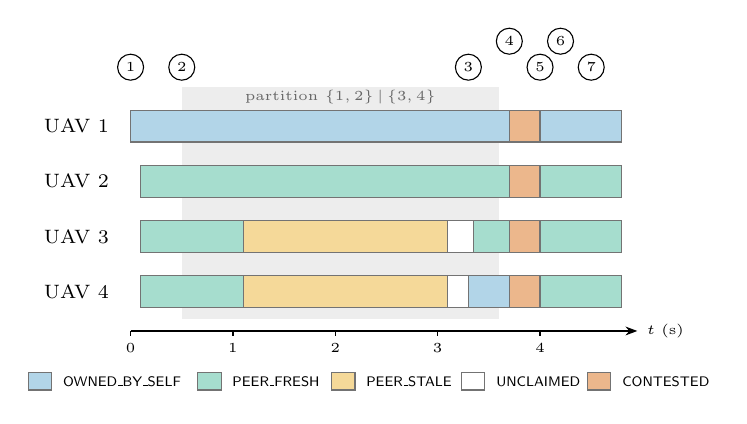
\begin{tikzpicture}[font=\scriptsize, >={Stealth[length=1.5mm]},
  ev/.style={circle, draw, inner sep=0.5pt, font=\tiny, fill=white, minimum size=3.3mm}]
  \foreach \uid/\ly in {1/2.1, 2/1.4, 3/0.7, 4/0.0}
    \node[anchor=east] at (1.15,\ly) {UAV \uid};
  \begin{scope}[xshift=1.3cm, x=1.3cm, y=1cm]
    % partition interval
    \fill[black!7] (0.5,-0.35) rectangle (3.6,2.6);
    \node[font=\tiny, black!60] at (2.05,2.47) {partition $\{1,2\}\,|\,\{3,4\}$};
    \def\sbseg#1#2#3#4{\filldraw[fill=#4, draw=black!55] (#1,#3-0.2) rectangle (#2,#3+0.2);}
    % UAV 1
    \sbseg{0.0}{3.7}{2.1}{cDist!30}
    \sbseg{3.7}{4.0}{2.1}{cCent!45}
    \sbseg{4.0}{4.8}{2.1}{cDist!30}
    % UAV 2
    \sbseg{0.1}{3.7}{1.4}{cGreen!35}
    \sbseg{3.7}{4.0}{1.4}{cCent!45}
    \sbseg{4.0}{4.8}{1.4}{cGreen!35}
    % UAV 3
    \sbseg{0.1}{1.1}{0.7}{cGreen!35}
    \sbseg{1.1}{3.1}{0.7}{cOrange!40}
    \sbseg{3.1}{3.35}{0.7}{white}
    \sbseg{3.35}{3.7}{0.7}{cGreen!35}
    \sbseg{3.7}{4.0}{0.7}{cCent!45}
    \sbseg{4.0}{4.8}{0.7}{cGreen!35}
    % UAV 4
    \sbseg{0.1}{1.1}{0.0}{cGreen!35}
    \sbseg{1.1}{3.1}{0.0}{cOrange!40}
    \sbseg{3.1}{3.3}{0.0}{white}
    \sbseg{3.3}{3.7}{0.0}{cDist!30}
    \sbseg{3.7}{4.0}{0.0}{cCent!45}
    \sbseg{4.0}{4.8}{0.0}{cGreen!35}
    % event markers
    \foreach \evx/\evn/\evy in {0.0/1/2.85, 0.5/2/2.85, 3.3/3/2.85, 3.7/4/3.18, 4.0/5/2.85, 4.2/6/3.18, 4.5/7/2.85}
      \node[ev] at (\evx,\evy) {\evn};
    % time axis
    \draw[->] (0,-0.5) -- (4.95,-0.5) node[right, font=\tiny] {$t$ (s)};
    \foreach \x in {0,1,2,3,4} {
      \draw (\x,-0.5) -- (\x,-0.56);
      \node[font=\tiny, below] at (\x,-0.54) {\x};
    }
  \end{scope}
  % legend
  \foreach \swatch/\legendtext/\lx in {cDist!30/{OWNED\_BY\_SELF}/0.0, cGreen!35/{PEER\_FRESH}/2.15,
      cOrange!40/{PEER\_STALE}/3.85, white/{UNCLAIMED}/5.5, cCent!45/{CONTESTED}/7.1} {
    \filldraw[fill=\swatch, draw=black!55] (\lx,-1.25) rectangle ++(0.3,0.22);
    \node[anchor=west, font=\tiny\sffamily] at (\lx+0.32,-1.14) {\legendtext};
  }
\end{tikzpicture}}
\caption{Each UAV's own view of Task~19 in the 2+2 split-brain demonstration.
Events: (1)~UAV~1 claims; (2)~partition; (3)~UAV~4 claims after its copy
expired (split brain); (4)~reconnection makes both claims visible;
(5)~independent reconciliation selects UAV~1; (6)~UAV~4's release delivered;
(7)~UAV~4 claims Task~29.}
\label{fig:splitbrain}
\end{figure}

\subsection{Identical awareness, opposite outcomes}
\label{sec:awareness}

We swept the communication range from 30 to 130 (11 values, 20 seeds, both
modes; 440 runs) with the region jammer active and UAV~2 failing at $t=4$\,s
(Fig.~\ref{fig:range}). \textbf{The centralized coordinator failed 68 of 220
missions; the distributed protocol failed none.} A failed central mission is
not a partial one: it completes 19 of 20 tasks and then spends the rest of its
300\,s budget holding the last task assigned to an aircraft that has stopped
(297.4 task-seconds stranded at range~30, against 1.8 for the distributed
mode).
Detection, however, is \emph{identical} in the two modes: in all 220 seed
pairs the two modes agree on whether the loss was ever declared (undetected
in 20/20 seeds at ranges 30--40, 18 at~50, 8 at~60, 2 at~70, none from~80).
The 68 central failures are exactly the 68 runs in which the loss went
undetected. What separates the modes is not what they know but whether acting
on it required agreement. Above range~60 the
distributed mode is flat (12.43\,s, 1.7 task-seconds stranded, 0.04
double-booked), so its behaviour stops depending on connectivity well before
central control stops failing.

\begin{figure}[t]
\centering
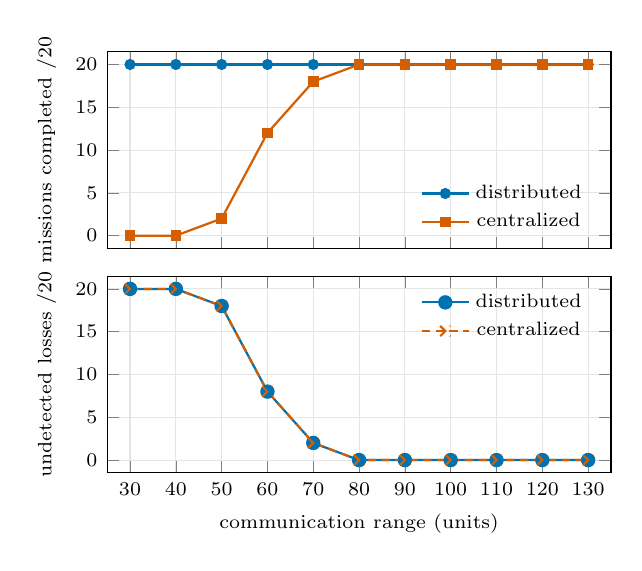
\begin{tikzpicture}
\begin{groupplot}[
  group style={group size=1 by 2, vertical sep=0.35cm, xticklabels at=edge bottom,
               xlabels at=edge bottom},
  scale only axis, width=6.4cm, height=2.5cm,
  xmin=25, xmax=135, xtick={30,40,...,130},
  ymin=-1.5, ymax=21.5, ytick={0,5,10,15,20},
  tick label style={font=\scriptsize}, label style={font=\scriptsize},
  legend style={font=\scriptsize, draw=none, fill=none},
  grid=major, grid style={black!10},
  xlabel={communication range (units)}]
\nextgroupplot[ylabel={missions completed /20}, legend pos=south east]
  \addplot[cDist, thick, mark=*, mark size=1.6pt] coordinates
    {(30,20)(40,20)(50,20)(60,20)(70,20)(80,20)(90,20)(100,20)(110,20)(120,20)(130,20)};
  \addlegendentry{distributed}
  \addplot[cCent, thick, mark=square*, mark size=1.5pt] coordinates
    {(30,0)(40,0)(50,2)(60,12)(70,18)(80,20)(90,20)(100,20)(110,20)(120,20)(130,20)};
  \addlegendentry{centralized}
\nextgroupplot[ylabel={undetected losses /20}, legend pos=north east]
  \addplot[cDist, thick, mark=*, mark size=2.2pt] coordinates
    {(30,20)(40,20)(50,18)(60,8)(70,2)(80,0)(90,0)(100,0)(110,0)(120,0)(130,0)};
  \addlegendentry{distributed}
  \addplot[cCent, thick, densely dashed, mark=x, mark size=2.6pt] coordinates
    {(30,20)(40,20)(50,18)(60,8)(70,2)(80,0)(90,0)(100,0)(110,0)(120,0)(130,0)};
  \addlegendentry{centralized}
\end{groupplot}
\end{tikzpicture}
\caption{Range sweep with a region jammer and a fail-stop (440 paired runs).
Top: mission completion. Bottom: aircraft that stopped and were never
declared. The curves coincide: identical awareness, opposite outcomes.}
\label{fig:range}
\end{figure}

\subsection{The quorum floor: a loss that cannot be declared}
\label{sec:floor}

A robustness sweep over 432 configurations produced no crashes but 108
incomplete missions, \emph{all} centralized. The minimal case is two aircraft
(Table~\ref{tab:floor}; presets \code{demo-quorum-floor} and
\code{baseline-quorum-floor}). By Proposition~\ref{prop:floor}, the survivor is the
only witness and can never declare its peer. Both modes are equally blind.
Central reassignment waits for a declaration that cannot arrive and never
finishes, while the distributed survivor re-claims the work when its lease
copy expires. A third aircraft restores the quorum and both modes recover,
which confirms that the floor is about witness count, not the control model.
In short, \emph{consensus-free recovery keeps working in exactly the
conditions that make consensus impossible.}

\begin{table}[t]
\caption{Quorum floor: one aircraft stops}
\label{tab:floor}
\centering
\footnotesize
\begin{tabular}{@{}clcccl@{}}
\toprule
UAVs & Mode & Declared & Undetected & Tasks & Mission \\
\midrule
2 & centralized & 0 & 1 & 2/3 & never finishes \\
2 & distributed & 0 & 1 & 3/3 & 10.75\,s \\
3 & centralized & 1 & 0 & 3/3 & completed \\
3 & distributed & 1 & 0 & 3/3 & completed \\
\bottomrule
\end{tabular}
\end{table}

\subsection{The price of availability, and the operator's dial}
\label{sec:price}

Availability is not free. In a 480-run lease sweep ($L\in[0.5,6]$\,s, range
50, jammer, no fail-stop; Fig.~\ref{fig:price}a) all runs completed, but
\emph{the two modes fail in opposite directions}. Central control never
double-booked in this sweep, but it handed work to aircraft it could not
reach: 4.79 task-seconds stranded on average, falling by a factor of 864 as
the lease grows. Replicated ownership stranded nothing and paid 0.29
task-seconds of double booking during the partition. That cost falls from
0.51 to 0.25 and then plateaus, because a replica that cannot hear the owner
re-claims once its own copy expires, however long the lease. Zero central
double booking is an observation for this configuration, not a structural
guarantee: the fleet study below found brief overlap involving a stopped UAV.

The operator's degradation policy moves the mission along this trade-off
(420 runs; Fig.~\ref{fig:price}b,c). \stt{HOLD} removes 64\% of double
booking (0.323$\rightarrow$0.116 task-seconds) and eliminates it from range~70
upwards, at the cost of 59\% longer missions (10.71$\rightarrow$17.06\,s). An
uncontracted swarm and \stt{CONTINUE} agree to three decimal places on every
metric across 280 runs, which confirms by measurement the invariant that a
contract only adds restraint. Which policy is right depends on the mission,
which is why the choice belongs to the operator rather than to the code.

\begin{figure*}[t]
\centering
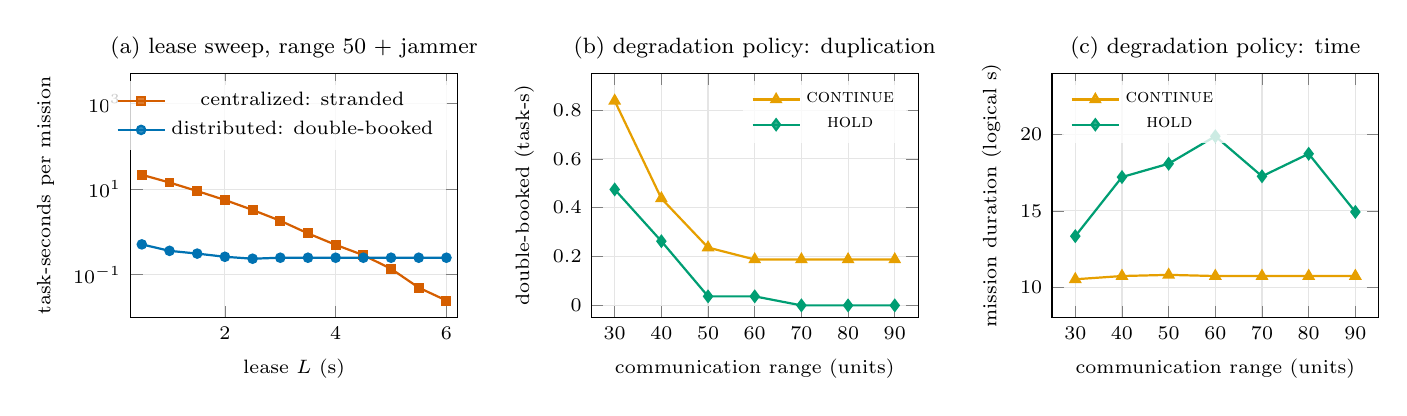
\begin{tikzpicture}
\begin{groupplot}[
  group style={group size=3 by 1, horizontal sep=1.7cm},
  scale only axis, width=4.15cm, height=3.1cm,
  tick label style={font=\scriptsize}, label style={font=\scriptsize},
  title style={font=\footnotesize, yshift=-1ex},
  legend style={font=\scriptsize, draw=none, fill=white, fill opacity=0.8, text opacity=1},
  grid=major, grid style={black!10}]
\nextgroupplot[title={(a) lease sweep, range 50 + jammer},
  xlabel={lease $L$ (s)}, ylabel={task-seconds per mission},
  ymode=log, ymin=0.01, ymax=5000, xmin=0.3, xmax=6.2, legend pos=north east]
  \addplot[cCent, thick, mark=square*, mark size=1.4pt] coordinates
    {(0.5,21.600)(1.0,14.250)(1.5,9.000)(2.0,5.575)(2.5,3.263)(3.0,1.825)
     (3.5,0.925)(4.0,0.500)(4.5,0.287)(5.0,0.138)(5.5,0.050)(6.0,0.025)};
  \addlegendentry{centralized: stranded}
  \addplot[cDist, thick, mark=*, mark size=1.5pt] coordinates
    {(0.5,0.512)(1.0,0.362)(1.5,0.312)(2.0,0.263)(2.5,0.237)(3.0,0.250)
     (3.5,0.250)(4.0,0.250)(4.5,0.250)(5.0,0.250)(5.5,0.250)(6.0,0.250)};
  \addlegendentry{distributed: double-booked}
\nextgroupplot[title={(b) degradation policy: duplication},
  xlabel={communication range (units)}, ylabel={double-booked (task-s)},
  ymin=-0.05, ymax=0.95, xmin=25, xmax=95, xtick={30,40,...,90}, legend pos=north east]
  \addplot[cOrange, thick, mark=triangle*, mark size=1.9pt] coordinates
    {(30,0.838)(40,0.438)(50,0.237)(60,0.188)(70,0.188)(80,0.188)(90,0.188)};
  \addlegendentry{\textsc{continue}}
  \addplot[cGreen, thick, mark=diamond*, mark size=1.9pt] coordinates
    {(30,0.475)(40,0.263)(50,0.037)(60,0.037)(70,0.000)(80,0.000)(90,0.000)};
  \addlegendentry{\textsc{hold}}
\nextgroupplot[title={(c) degradation policy: time},
  xlabel={communication range (units)}, ylabel={mission duration (logical s)},
  ymin=8, ymax=24, xmin=25, xmax=95, xtick={30,40,...,90}, legend pos=north west]
  \addplot[cOrange, thick, mark=triangle*, mark size=1.9pt] coordinates
    {(30,10.512)(40,10.725)(50,10.800)(60,10.725)(70,10.725)(80,10.725)(90,10.725)};
  \addlegendentry{\textsc{continue}}
  \addplot[cGreen, thick, mark=diamond*, mark size=1.9pt] coordinates
    {(30,13.338)(40,17.212)(50,18.087)(60,19.887)(70,17.262)(80,18.738)(90,14.925)};
  \addlegendentry{\textsc{hold}}
\end{groupplot}
\end{tikzpicture}
\caption{The price of availability. (a)~Central control strands work it
cannot reach; replicated ownership instead double-books briefly during a
partition (480 runs, all completed). (b,c)~The operator's \stt{HOLD} policy
trades duplication for time (420 runs, 20 seeds per point; uncontracted runs
coincide with \stt{CONTINUE} and are not drawn). Lines between points are
drawn for readability only.}
\label{fig:price}
\end{figure*}

\subsection{The detection floor: a cliff for one layout, a gradient for many}
\label{sec:detect}

Failure detection needs a quorum of peers that can still hear one another,
and nothing guarantees that one exists. For the default task layout (seed
2026, no jammer), detection fails as a cliff: the loss is declared at every
tested range from 76 to 130 and at none from 75 down, yet all 20 tasks still
complete because leases expire on their own. Across 20 task-placement seeds the same detector
degrades gradually instead (18/20 losses undetected at range~50, 8 at~60, 2
at~70, none from~80), with or without the jammer. Both shapes are real; the
cliff belongs to one geometry. Either way, \emph{no mission-level number
reveals that an aircraft is gone}, which is precisely what makes undetected
loss dangerous and why we report it as its own metric.

\subsection{Fleet size, network regime, layout and fault timing}
\label{sec:generality}

A paired fleet/network study (240 runs; Table~\ref{tab:gen}) scales the area
side as $100\sqrt{N/4}$ with two tasks per UAV, fails UAV~2 at $t=4$\,s and
caps missions at 30\,s. In the sparse regimes the distributed mode finished
when its paired central run timed out in 18/20 (four UAVs) and 19/20 (six
UAVs) seeds, never the reverse. Central control showed small but non-zero
overlap in four high-range runs. A trace shows Task~5 claimed both by a
responsive UAV and by the stopped UAV~2: claim overlap after reassignment,
not two aircraft flying.

\begin{table}[t]
\caption{Paired fleet and network comparison (20 seeds per cell; means in
task-seconds; D = distributed, C = centralized)}
\label{tab:gen}
\centering
\footnotesize
\setlength{\tabcolsep}{3.2pt}
\begin{tabular}{@{}clcccccc@{}}
\toprule
& & \multicolumn{2}{c}{Complete} & \multicolumn{2}{c}{Stranded} & \multicolumn{2}{c}{Overlap} \\
\cmidrule(lr){3-4}\cmidrule(lr){5-6}\cmidrule(l){7-8}
$N$ & Network & D & C & D & C & D & C \\
\midrule
4 & high range & 20 & 20 & 0.03 & 6.65  & 0.00 & 0.07 \\
4 & sparse     & 20 & 2  & 0.28 & 27.38 & 0.72 & 0.00 \\
4 & sparse+jam & 20 & 2  & 0.60 & 27.40 & 1.73 & 0.00 \\
6 & high range & 20 & 20 & 0.03 & 11.25 & 0.00 & 0.03 \\
6 & sparse     & 20 & 1  & 0.07 & 32.73 & 0.12 & 0.00 \\
6 & sparse+jam & 20 & 1  & 0.17 & 32.73 & 0.78 & 0.00 \\
\bottomrule
\end{tabular}
\end{table}

A second study (960 runs; Table~\ref{tab:robust}) adds a centred-ring starting
layout and moves the fault to $t=2$ or $t=6$\,s. The distributed mode
completed all 480 of its runs and the centralized mode 337. The gap depends
strongly on geometry and fault time: an early fault in the default layout
gave 0/20 central completions in every sparse condition, while a late fault
on the ring often gave 20/20. The ring also produces fewer components in
sparse runs (mean maximum 1.43 vs.\ 3.21). Late-fault ring runs need a
caveat: in 81 of 960 rows the mission finished \emph{before} the scheduled
fault. Restricted to the 75 pairs in which both modes actually experienced
the fault, both modes completed every run except under six-UAV sparse plus
jammer, where the distributed mode completed 14/14 against 12/14. The jammer raised
mean distributed overlap from 0.33 to 0.94 task-seconds (central:
0.03$\rightarrow$0.02).

\begin{table}[t]
\caption{Layout and fault-time sensitivity: missions completed out of 20,
D\,/\,C (960 paired runs)}
\label{tab:robust}
\centering
\footnotesize
\setlength{\tabcolsep}{4pt}
\begin{tabular}{@{}cccccc@{}}
\toprule
$N$ & Layout & Fault & High range & Sparse & Sparse+jam \\
\midrule
4 & default & 2\,s & 20\,/\,20 & 20\,/\,0  & 20\,/\,0  \\
4 & default & 6\,s & 20\,/\,20 & 20\,/\,19 & 20\,/\,16 \\
4 & ring    & 2\,s & 20\,/\,20 & 20\,/\,10 & 20\,/\,10 \\
4 & ring    & 6\,s$^\dagger$ & 20\,/\,20 & 20\,/\,20 & 20\,/\,20 \\
6 & default & 2\,s & 20\,/\,20 & 20\,/\,0  & 20\,/\,0  \\
6 & default & 6\,s & 20\,/\,20 & 20\,/\,18 & 20\,/\,18 \\
6 & ring    & 2\,s & 20\,/\,20 & 20\,/\,4  & 20\,/\,4  \\
6 & ring    & 6\,s$^\dagger$ & 20\,/\,20 & 20\,/\,20 & 20\,/\,18 \\
\bottomrule
\end{tabular}

\vspace{2pt}
{\scriptsize $^\dagger$Some runs finished before the scheduled fault; see
text for the fault-exposed subset.\par}
\end{table}

% =============================================================================
\section{Live Mission on ArduPilot SITL}
\label{sec:live}

For the EUDIS Defence Hackathon (Challenge~2, \emph{Swarm Coordination and
Autonomous Operations}), the claim protocol was taken out of the simulator and
used to fly a mission on ArduPilot~\cite{ardupilot}. One ground-node laptop
runs one receiver-local agent per aircraft and commands each autopilot in
GUIDED mode over MAVLink~\cite{koubaa2019mavlink}. Vehicles may be SITL,
physical, or both, in one local frame georeferenced at the USRL Orounda
airfield. Inter-UAV links are emulated with the same \code{CommunicationGraph},
fed by real telemetry positions; claim gossip, leases and lowest-identifier
reconciliation are the simulator's own code. This harness runs on wall-clock
time and is \emph{not} deterministic, so a live run is reported as an
observation, never as a measured result.

\subsection{Ground node and safety envelope}

Aircraft have one of two roles: ISR (search and detection) or LM
(loitering-munition role for engagement; here an ordinary multirotor whose
release is simulated). Each role has an altitude band: ISR 5--25\,m and LM 30--60\,m, under a
60\,m ceiling and a 400\,m operating radius. The two roles are therefore
vertically separated by construction. Every setpoint is checked against the
vehicle's band and radius before it is stored. The ground node never arms a
physical aircraft: a safety pilot takes off and hands over by selecting
GUIDED. Any mode change the ground node did not command is treated as a final
takeover, after which the vehicle is never commanded again in that run.
Commands are re-sent until they take effect, heartbeats go out at 1\,Hz so
that autopilot failsafes fire only if the ground node is really gone,
telemetry older than 2\,s is never treated as current, and an interrupt
returns every vehicle to launch. The autopilot's own geofence and failsafes
remain the safety net.

\subsection{Search as claimable sectors}

The operator's convex search area (default $240\times160$\,m) is cut into
strips. Each strip is a task in the claim protocol: ISR aircraft claim sectors
and fly boustrophedon lanes~\cite{choset2000boustrophedon} at their own
altitude, spaced so that consecutive camera footprints overlap by 20\% (a Pi
Camera v2 sees about 24\,m across at 20\,m, roughly 3.8\,cm per pixel). An ISR
publishes completion at the last waypoint. Every participating aircraft
relays evidence.

\subsection{Perception, geolocation and target discovery}

A detection is a pixel $(u,v)$ in a $W\times H$ frame from a nadir camera with
fields of view $\theta_h,\theta_v$. At height $h$ it maps to the ground offset
\begin{equation}
  \Delta_{\mathrm{right}} = \tfrac{2u-W}{W}\,h\tan\tfrac{\theta_h}{2},\quad
  \Delta_{\mathrm{fwd}} = \tfrac{H-2v}{H}\,h\tan\tfrac{\theta_v}{2},
\end{equation}
rotated by the aircraft heading. Attitude is assumed level; at search speed a
few degrees of pitch move the estimate by $h\tan(\text{pitch})$, a metre or
two at 20\,m. Each ISR fuses its sightings into local tracks and publishes an
immutable \emph{target report}, which floods like any other evidence and
becomes a new engagement task. Two ISRs may report one object before hearing
each other. Among the reports a UAV knows, one lying within 10\,m of a report
with a lower task identifier is treated as its duplicate, so every receiver
with the same evidence engages the same canonical report. SITL ISRs use a
synthetic camera with misses and pixel noise that never reveals target
identity. Physical ISRs stream version-1 JSON-Lines observations over UDP from
an on-board detector, geolocated with the aircraft's telemetry \emph{at the
frame's timestamp}, which requires the on-board computer's clock to be
synchronised with the ground node. Camera health is evidence too: a camera that reports
\emph{stalled}, or sends nothing for 3\,s, is shown as silent, and silence
never counts as an empty scene.

\subsection{Human-confirmed engagement}
\label{sec:engage}

Each target report is an engagement task claimed by LMs through the same
protocol. The owner transits at 40\,m and \emph{holds 30\,m short until the
operator confirms} on the map; \emph{Abort} withdraws the target for the rest
of the run. After confirmation the LM descends to 30\,m over the aim point,
dwells 3\,s and performs a \emph{simulated} release, but only if it still owns
the claim at that instant. The release publishes completion, and the LM
returns to launch, spent. Nothing leaves the aircraft; on a physical LM the
release pulses an LED or buzzer on an autopilot relay. Both operator
decisions attach to the \emph{object}, so a duplicate report inherits them. If
the LM owning a confirmed target fails, its claim expires after the lease and
the next free LM takes over under the same confirmation. Physical LMs act as
a reserve: a reserve claims a target only after it has stayed unclaimed for
8\,s in its own view, a receiver-local role preference that keeps the
expensive asset back while expendable ones are free.

\subsection{Advisory QAOA assignment planner}
\label{sec:qaoa}

The challenge asks for optimisation using quantum simulation. When the set of
idle LMs $\mathcal{L}$ or open targets $\mathcal{T}$ changes, the ground node
solves the assignment as a QUBO~\cite{lucas2014ising} over
$x_{\ell t}\in\{0,1\}$. For $|\mathcal{L}|\ge|\mathcal{T}|$,
\begin{equation}
\begin{split}
  E(x) ={}& \sum_{\ell,t} d_{\ell t}x_{\ell t}
  + P\sum_{t}\Bigl(1-\sum_{\ell}x_{\ell t}\Bigr)^{2}\\
  &+ P\sum_{\ell}\sum_{t<t'}x_{\ell t}x_{\ell t'},
\end{split}
  \label{eq:qubo}
\end{equation}
with straight-line distances $d_{\ell t}$ and $P=2\max d+1$; the roles of the
two constraints swap when targets outnumber LMs. We simulate the quantum
alternating operator ansatz~\cite{hadfield2019qaoa} on a NumPy statevector.
The initial state is a product of W-states, one per target (an equal
superposition of ``exactly one LM''). Each of $p=3$ layers applies the cost
phase $e^{-i\gamma_k\tilde E}$ followed by an XY ring
mixer~\cite{wang2020xy} inside each target's group, which never leaves the
one-hot subspace. $\tilde E$ is $E$ normalised over that subspace. Angles
follow a linear ramp chosen by grid search and are then refined coordinate by
coordinate. The answer is the best feasible bitstring among the 16 most
probable, as repeated measurement would give. A transverse-field mixer was
tried first and abandoned: on the $4\times3$ instance only 24 of 4,096
bitstrings are valid, and it placed about 0.1\% probability on the optimum.

The plan is \emph{advice}. Each LM adds 50\,m to every target except its
recommended one, and the claim protocol still decides who flies. The exact
optimum is computed by enumeration alongside every solve; classically, this
assignment problem is solvable in polynomial time by the Hungarian
method~\cite{kuhn1955hungarian}. Table~\ref{tab:qaoa} benchmarks
120 seeded random instances (LMs on the launch row, targets in the search
area). QAOA's readout matched the exact optimum in 118; the two misses cost
1.1\% and 2.4\% more than the optimum. The probability it places on the
optimum, however, is only 1.4--2.3 times that of the uniform initial state,
and it is \emph{comparable to sampling a valid assignment uniformly at
random} (lower at $3\times3$ and $4\times3$). At these sizes the 16-candidate
readout covers much of the reachable subspace (16 of 64 states at 12
qubits), so the match rate reflects classical post-selection as much as the
ansatz. There is no quantum advantage here, and we claim none. The value is
the formulation and an honest integration that keeps the quantum step off the
critical path.

\begin{table}[t]
\caption{QAOA planner versus exact optimum (20 seeded instances per size,
$p=3$). Size: LMs $\times$ targets. Opt.: readout equals the exact optimum. $P_{\mathrm{opt}}$:
probability QAOA places on the optimum. Baselines: uniform over the reachable
one-hot subspace (Unif.) and over valid assignments (Valid). Times on a
laptop CPU.}
\label{tab:qaoa}
\centering
\footnotesize
\setlength{\tabcolsep}{4pt}
\begin{tabular}{@{}ccccccc@{}}
\toprule
Size & Qubits & Opt. & $P_{\mathrm{opt}}$ & Unif. & Valid & Time (s) \\
\midrule
$2\times2$ & 4  & 20/20 & 0.514 & 0.250 & 0.500 & 0.01 \\
$3\times2$ & 6  & 20/20 & 0.208 & 0.111 & 0.167 & 0.04 \\
$4\times2$ & 8  & 20/20 & 0.107 & 0.063 & 0.083 & 0.06 \\
$3\times3$ & 9  & 20/20 & 0.085 & 0.037 & 0.167 & 0.08 \\
$5\times2$ & 10 & 19/20 & 0.056 & 0.040 & 0.050 & 0.11 \\
$4\times3$ & 12 & 19/20 & 0.034 & 0.016 & 0.042 & 0.28 \\
\bottomrule
\end{tabular}
\end{table}

\subsection{Observed runs}

All runs were on one development laptop with eight ArduCopter SITL instances,
and each was flown once.
\emph{Ring flight:} every vehicle reached its ring point within 3\,m at its
layer altitude and landed at its launch point.
\emph{Search with a fail-stop:} with \code{isr\_04} killed at 60\,s while
owning sector S3, two ISRs claimed S6 at once and the lower identifier kept
it; the first ISR free after S3's lease had expired took it over at 89.9\,s;
all six sectors were searched exactly once by 163\,s.
\emph{Full demonstration} (Table~\ref{tab:events}, Fig.~\ref{fig:map}): an ISR
inside an emulated jam zone detected the target while isolated, and its
report flooded out when its links returned. The first LM to engage was
fail-stopped by design; after its lease expired a second LM took the target,
held short until the operator confirmed, and released 0.3\,m from its aim
point (the geolocated estimate) and 0.1\,m from the object's true position.
The reserve LM engaged last, once the others were spent. All six sectors
were searched, all three targets were eliminated, and all eight aircraft
landed.

\begin{table}[t]
\caption{Event log excerpt, full SITL demonstration (one run, observed)}
\label{tab:events}
\centering
\footnotesize
\setlength{\tabcolsep}{3pt}
\begin{tabular}{@{}rlL{5.0cm}@{}}
\toprule
$t$ (s) & Vehicle & Event \\
\midrule
76.0  & isr\_02 & enters active jam zone \\
81.2  & isr\_02 & detects T20 while jammed \\
81.2  & planner & QAOA advice lm\_02$\rightarrow$T20 (= exact optimum) \\
81.6  & isr\_02 & links restored; report floods out \\
81.6  & lm\_02  & engages T20; fail-stop injected \\
93.6  & lm\_03  & engages T20 after lm\_02's lease expired \\
103.5 & lm\_03  & holds 30\,m short of T20 \\
130.3 & operator & confirms T20 on the map \\
140.8 & lm\_03  & simulated release, 0.3\,m from aim point \\
197.8 & lm\_01  & reserve engages T11 (others spent) \\
257.3 & lm\_01  & simulated release, 0.3\,m from aim point \\
\bottomrule
\end{tabular}
\end{table}

\begin{figure*}[t]
\centering
\subfloat[Holding short: the LM awaits \emph{Confirm strike}.]{%
  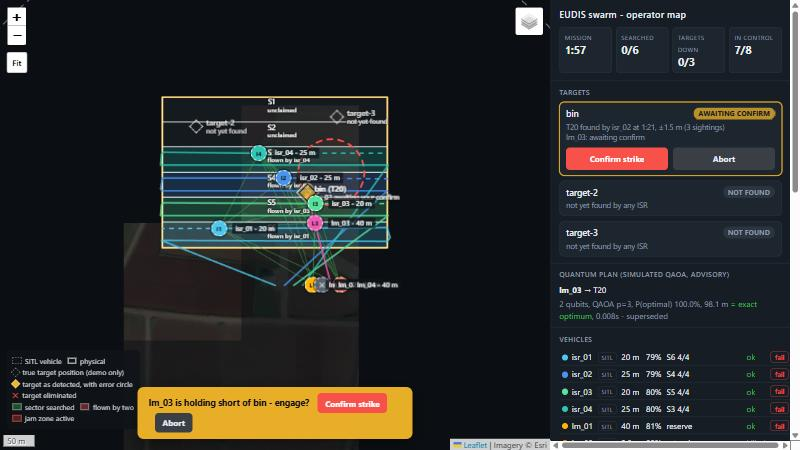
\includegraphics[width=0.49\textwidth]{figures/operator_map_confirm.jpg}%
  \label{fig:map:confirm}}\hfill
\subfloat[First target eliminated (release 0.1\,m from true position).]{%
  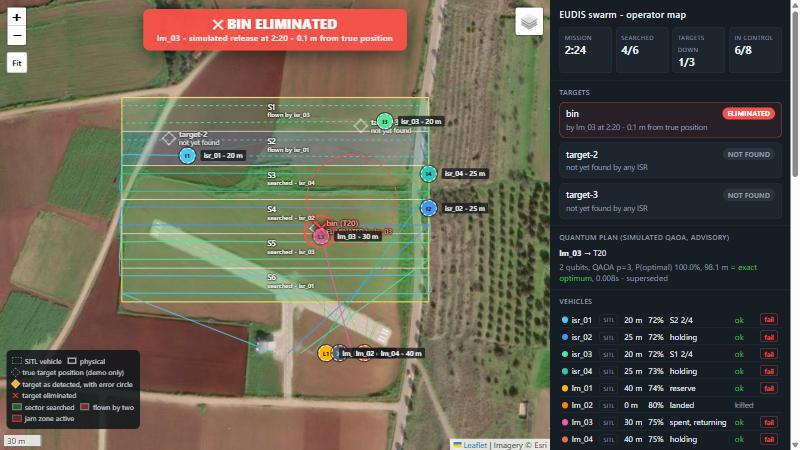
\includegraphics[width=0.49\textwidth]{figures/operator_map_eliminated.jpg}%
  \label{fig:map:elim}}\\[1mm]
\subfloat[Mission complete: 6/6 sectors searched, 3/3 targets eliminated, all
  aircraft returned.]{%
  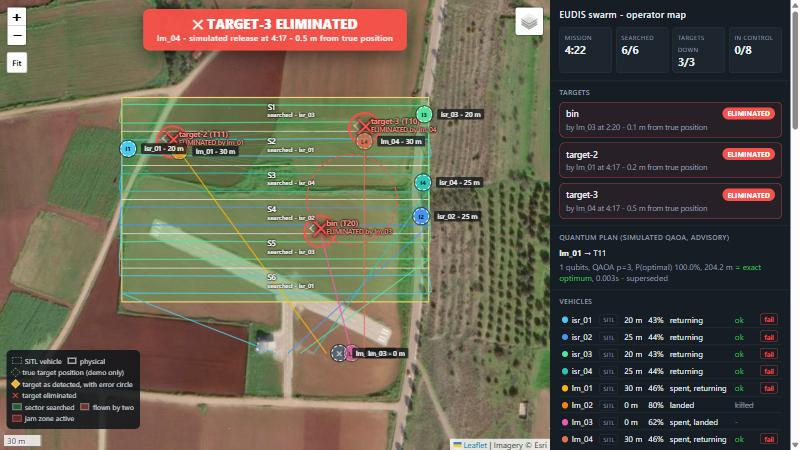
\includegraphics[width=0.49\textwidth]{figures/operator_map_mission_complete.jpg}%
  \label{fig:map:done}}
\caption{The operator map during the eight-vehicle SITL mission at USRL
Orounda (imagery \copyright\ Esri, map library Leaflet~\cite{leaflet}). Sectors
are tinted by the UAV flying or having searched them, red if two fly one at
once. Dashed diamonds mark true target positions for demonstration only; no
UAV sees them. Solid diamonds with error circles are geolocated estimates. The
side panel shows the latest advisory QAOA plan. \emph{Confirm} and
\emph{Abort} are the only controls by which the page can affect the mission.}
\label{fig:map}
\end{figure*}

\subsection{How wrong is the point-mass model?}
\label{sec:modelerror}

The simulator predicts motion with a point mass: constant speed, instant
acceleration, exact arrival. We flew the same 60\,m leg six times on one
ArduCopter SITL vehicle, giving the model the autopilot's own 10\,m/s so that
it had its best case (Table~\ref{tab:modelerror}). Real legs took 1.71 times
longer than predicted. Peak divergence, 34\,m on average, occurred at
5.8\,s, exactly when the model says the aircraft has arrived and stopped,
while the real one was still a third of the way back. Arrival error was small
(1.7\,m). This is why all simulated durations are reported as logical
seconds. Its effect on coordination decisions has not yet been measured.

\begin{table}[t]
\caption{Point-mass prediction vs.\ ArduCopter SITL, 60\,m leg (6 legs, one
vehicle; SITL is not reproducible, so ranges are shown)}
\label{tab:modelerror}
\centering
\footnotesize
\begin{tabular}{@{}lrrr@{}}
\toprule
& Min & Max & Mean \\
\midrule
Duration / model prediction & 1.53 & 1.76 & 1.71 \\
Worst position error during leg (m) & 25.25 & 37.26 & 34.43 \\
Arrival error (m) & 1.40 & 1.99 & 1.67 \\
\bottomrule
\end{tabular}
\end{table}

% =============================================================================
\section{Discussion and Limitations}
\label{sec:discussion}

\emph{What the evidence supports.} Within a deterministic, two-dimensional,
point-mass simulation with an abstract range/jammer link model,
receiver-local leases recover work in conditions where declaration-gated
reassignment cannot. The difference is not explained by awareness, because
detection is identical. Replicated ownership pays with transient double
booking, and the operator can trade it against time.

\emph{What it does not support.} (i)~\emph{RF:} the link model is analytical
and uncalibrated, and the threat sources concern GNSS, not inter-vehicle
links. (ii)~\emph{Absolute time:} durations are logical seconds under a
motion model whose error we measured at $1.7\times$. (iii)~\emph{Generality:}
the results cover a few scenario families (4--6 UAVs, two layouts, one
jammer geometry). The completion gap is highly sensitive to geometry and
fault timing (Table~\ref{tab:robust}). (iv)~\emph{Baseline:} our centralized
coordinator is one specific design, declaration-gated and greedy; a
coordinator that reassigned on silence alone would recover faster but would
also reassign work from healthy, merely partitioned aircraft, the failure
mode this work is built to avoid. (v)~\emph{Faults:} only fail-stop is modelled;
Byzantine behaviour, identity forgery, asymmetric links, latency, bandwidth
and simultaneous failures are out of scope. Flooding retains seen-state and
can grow as $O(mN^2)$ for $m$ messages. (vi)~\emph{EFSMs:} requested effects
have no dispatcher yet, and the coordination mode is advisory.
(vii)~\emph{Live mission:} the ground node hosts all agents in one process
with emulated inter-UAV links. Live runs are single observations. Fleet
telemetry does not yet drive the deterministic simulator through its vehicle
interface, and no physical aircraft or live perception stream has yet flown
the mission end to end. (viii)~\emph{QAOA:} no quantum advantage at this size;
its readout is substantially classical post-selection
(Section~\ref{sec:qaoa}).

\emph{Responsible use.} The engagement task in the live mission is a
demonstration of human authority in a coordination protocol, not a weapon. The
release is simulated and nothing leaves the aircraft. Every engagement
requires explicit operator confirmation per object, \emph{Abort} is final, a
release requires continuing ownership at that instant, and any pilot mode
change permanently removes the swarm's authority over that vehicle. The
software is a research prototype; it is not flight-certified and must not be
used to command real vehicles outside an authorised, supervised test range.

% =============================================================================
\section{Conclusion}
\label{sec:conclusion}

Silence is ambiguous, and in a contested RF environment it is the normal
case. We built a swarm-coordination protocol around that fact: each UAV acts
only on evidence it has received, ownership is a lease rather than a verdict,
conflicts created by partition are allowed and reconciled deterministically,
and failure declarations inform rather than gate recovery. In paired
simulations the distributed and centralized modes see exactly the same
losses, yet only the consensus-free mode keeps completing missions once the
network is sparse, jammed or too small for a quorum. The cost is transient
double booking, which the operator can buy down with a \stt{HOLD} policy.
The same protocol coordinates search and human-confirmed engagement on eight
autopilot SITL vehicles. Next steps are to drive the simulator from fleet
telemetry, to fly the mixed physical/SITL mission at the airfield, to run
agents in separate processes over real radios, to dispatch EFSM effects into
role and relay behaviour, and to replace the point-mass model with a
calibrated airframe model.

% =============================================================================
\section*{Acknowledgment}
% TODO: acknowledge team members who are not authors (e.g. perception and
% hardware/flight-operations work), mentors, and any sponsor or partner, in
% line with the organisers' rules on declared company backing.
The authors thank the organisers of the EUDIS Defence Hackathon 2026
(Cyprus). The on-board perception pipeline for the physical ISR aircraft,
based on VERA-MOT, is the work of [TODO: name], Team Teleforce. This work is
an independent team prototype; it is not affiliated with or endorsed by any
hackathon partner, sponsor or host.

\bibliographystyle{IEEEtran}
\bibliography{references}

% =============================================================================
\appendices

\section{Design Notebook}
\label{app:sketches}

Fig.~\ref{fig:sketches} reproduces the team's original design notebook pages
(2 and 10 August 2026), from which Figs.~\ref{fig:conops} and~\ref{fig:arch},
the network-loss states of Section~\ref{sec:model}, the failure and safety
behaviour of Section~\ref{sec:recovery} and the utility of
Eq.~\eqref{eq:cost} were developed. The photographs are cropped, with
illumination flattened for print and content unaltered.

\begin{figure*}[!p]
\centering
\subfloat[Operational problem definition and the autonomous swarm layer.]{%
  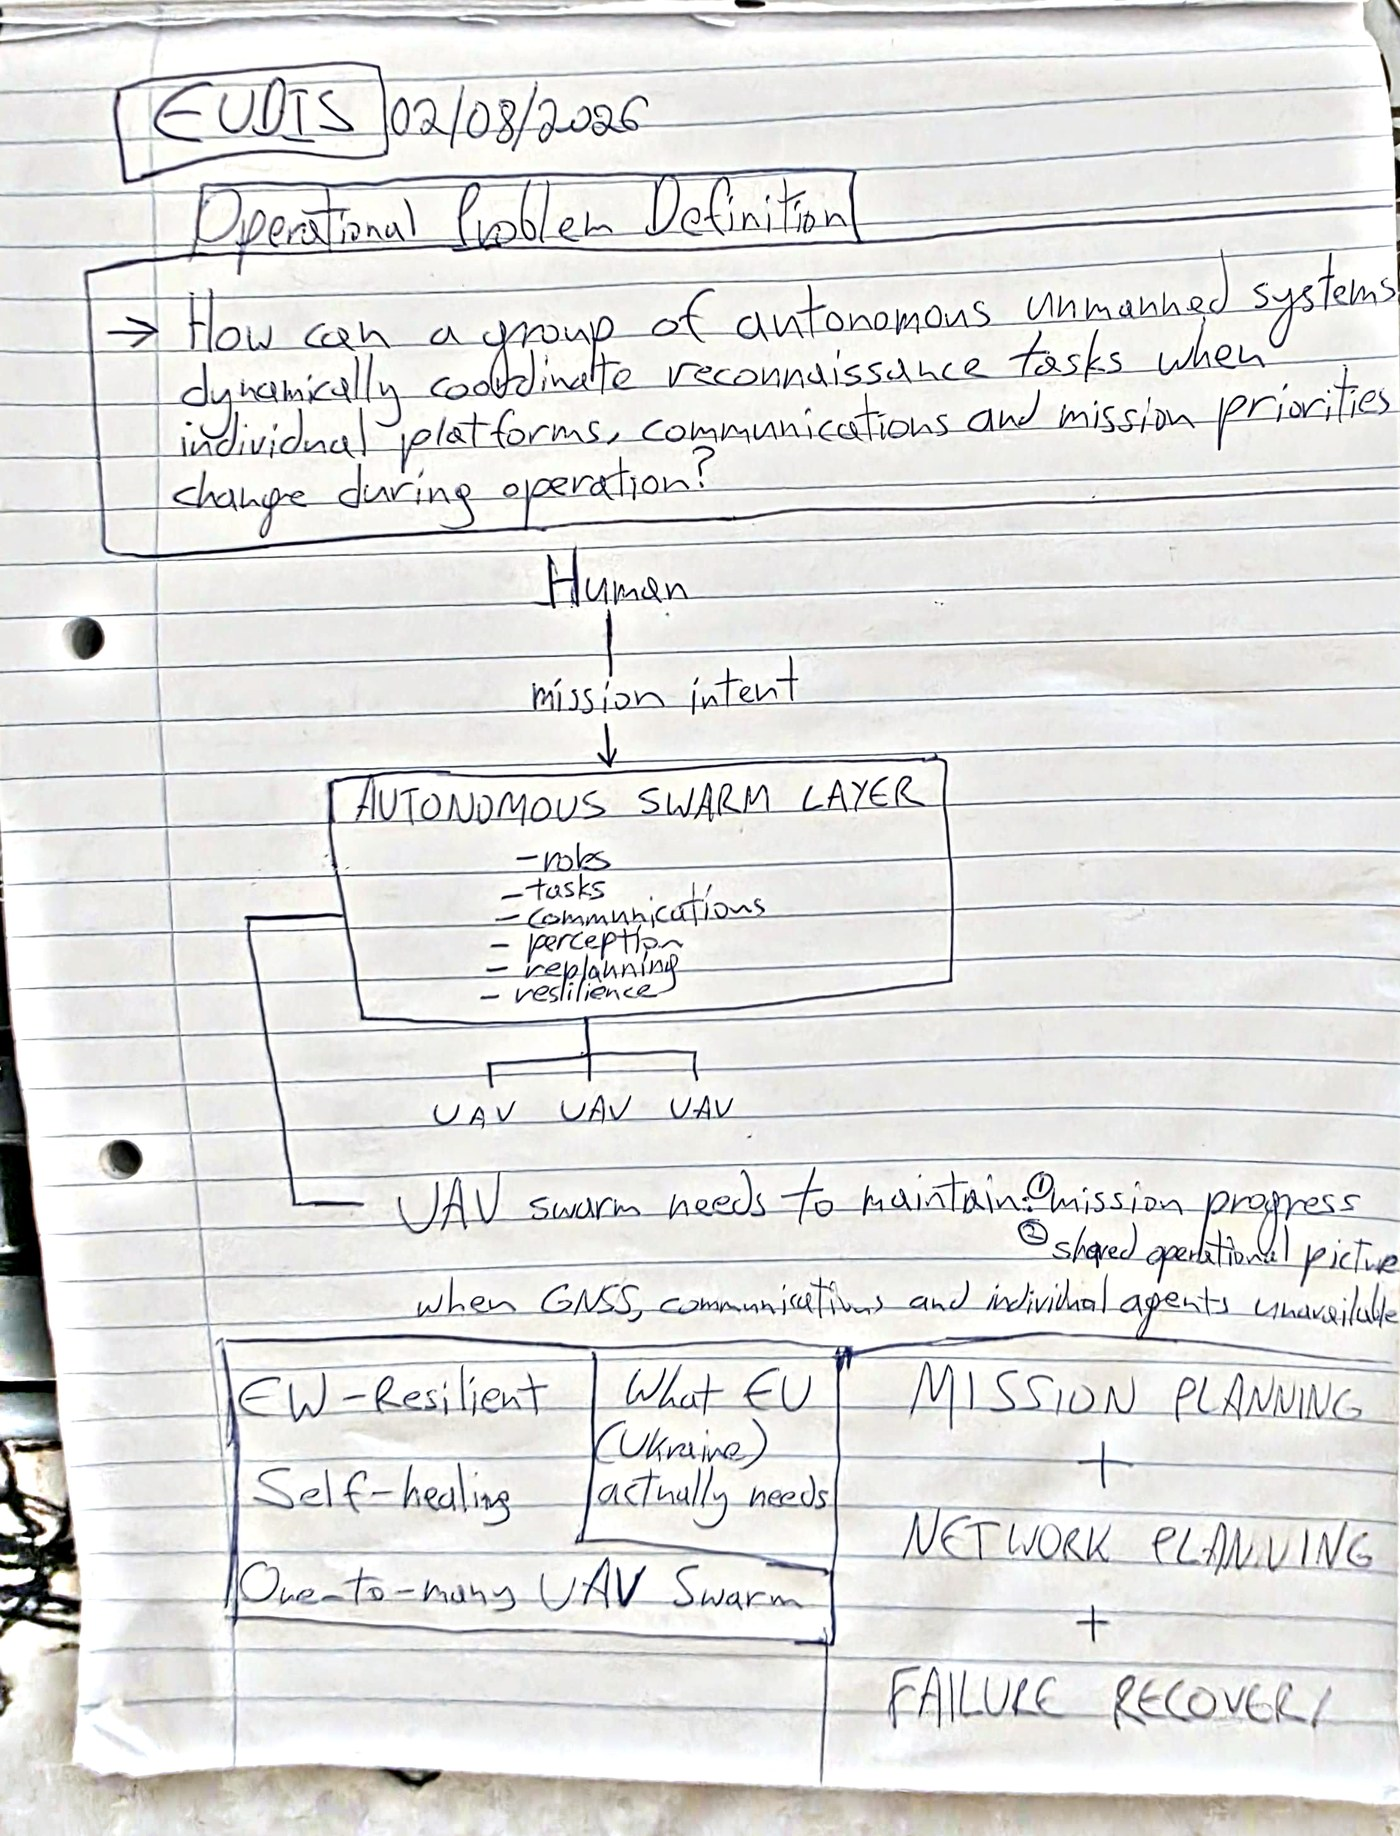
\includegraphics[width=0.31\textwidth]{figures/sketch_problem.jpg}}\hfill
\subfloat[CONOPS: main idea, scalability rules, architecture.]{%
  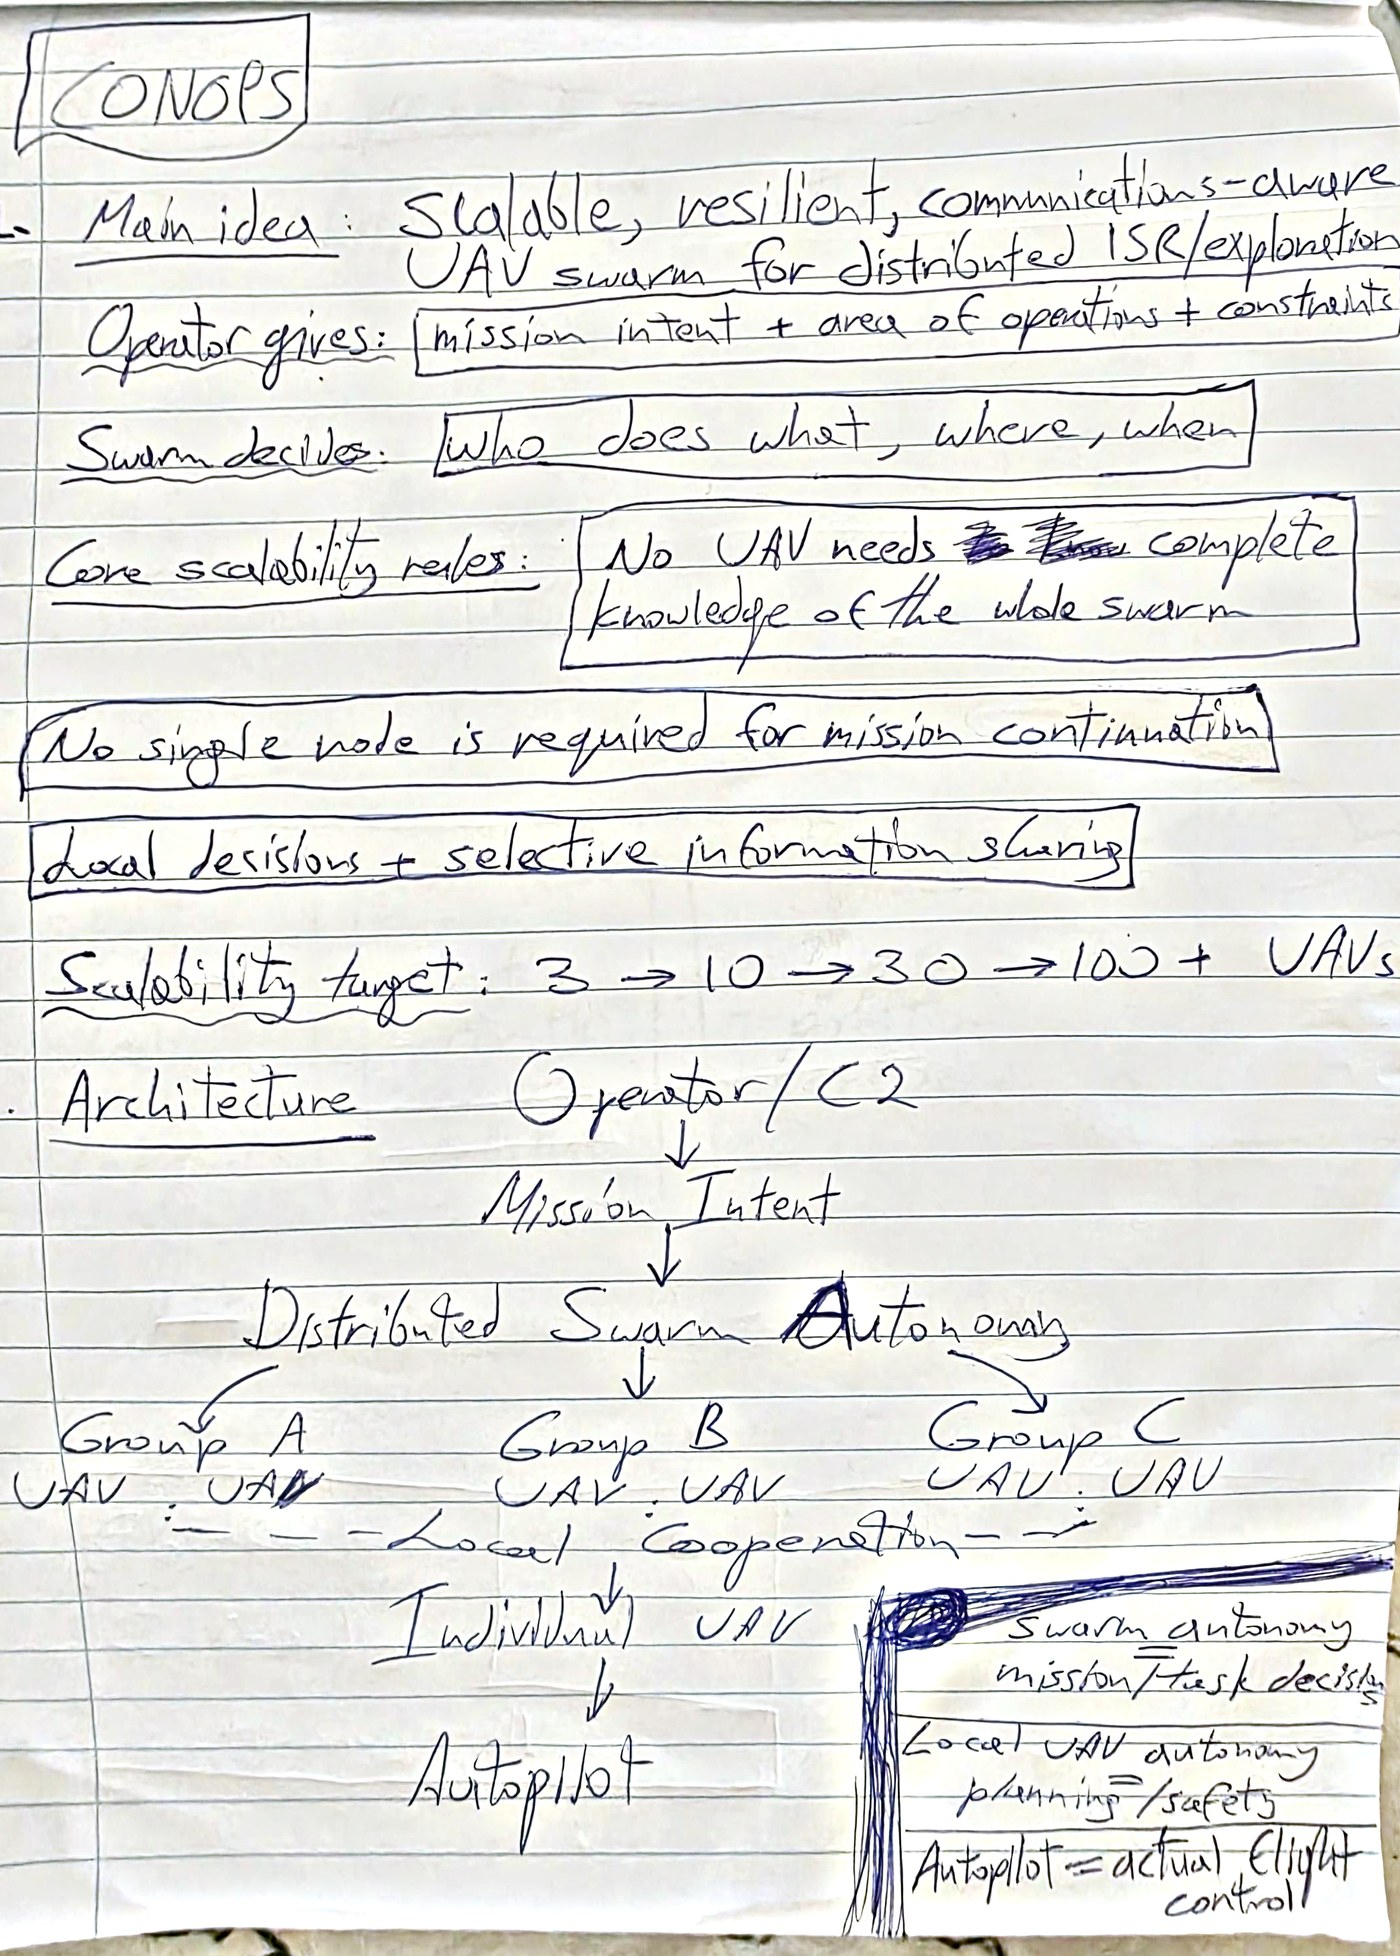
\includegraphics[width=0.31\textwidth]{figures/sketch_conops.jpg}}\hfill
\subfloat[Local state per UAV, message types, task-based operation.]{%
  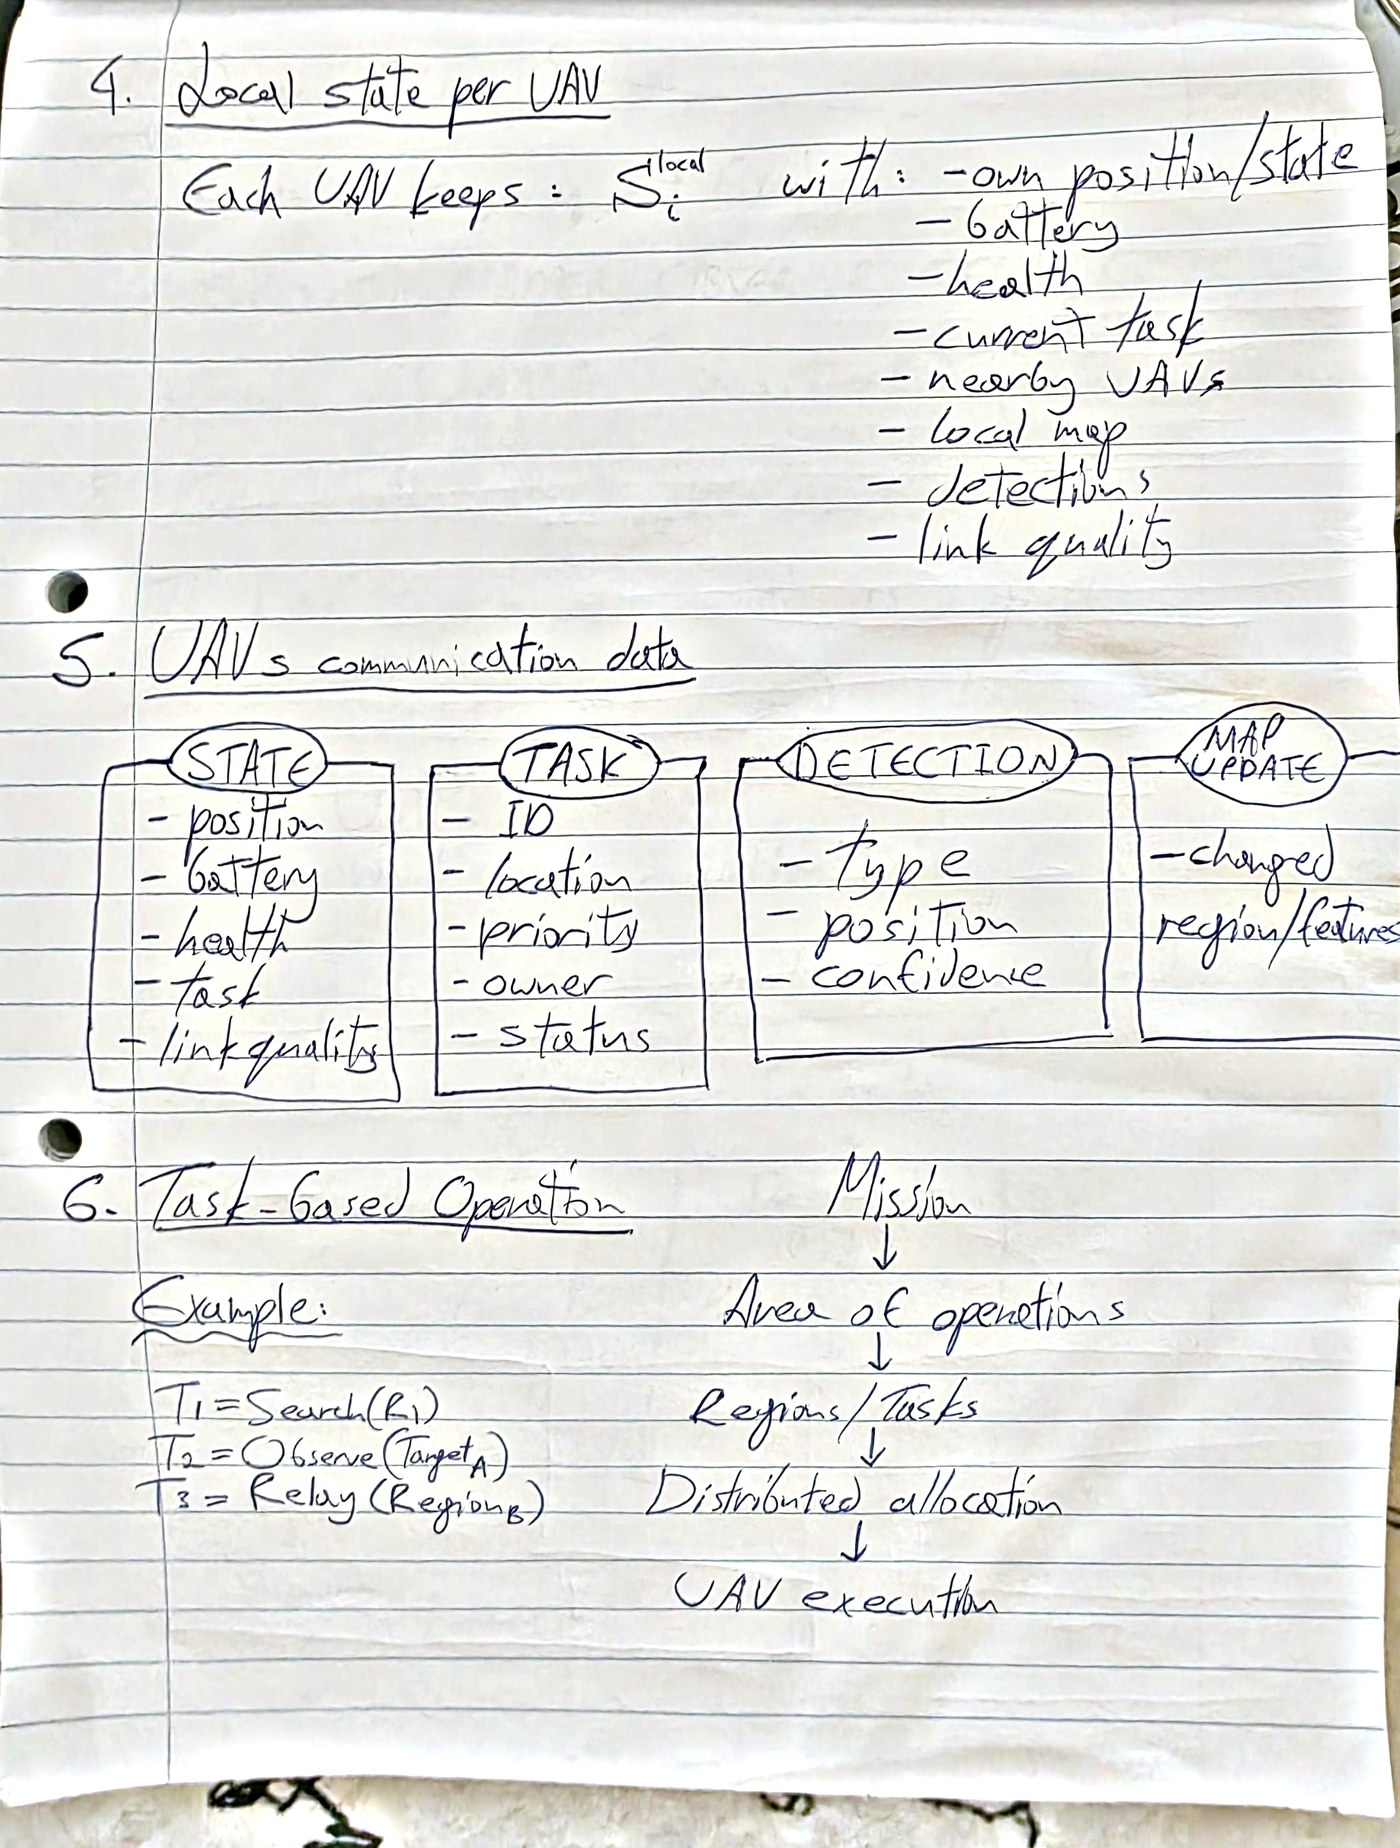
\includegraphics[width=0.31\textwidth]{figures/sketch_state_tasks.jpg}}\\[2mm]
\subfloat[Dynamic roles; communication graph; network loss is normal.]{%
  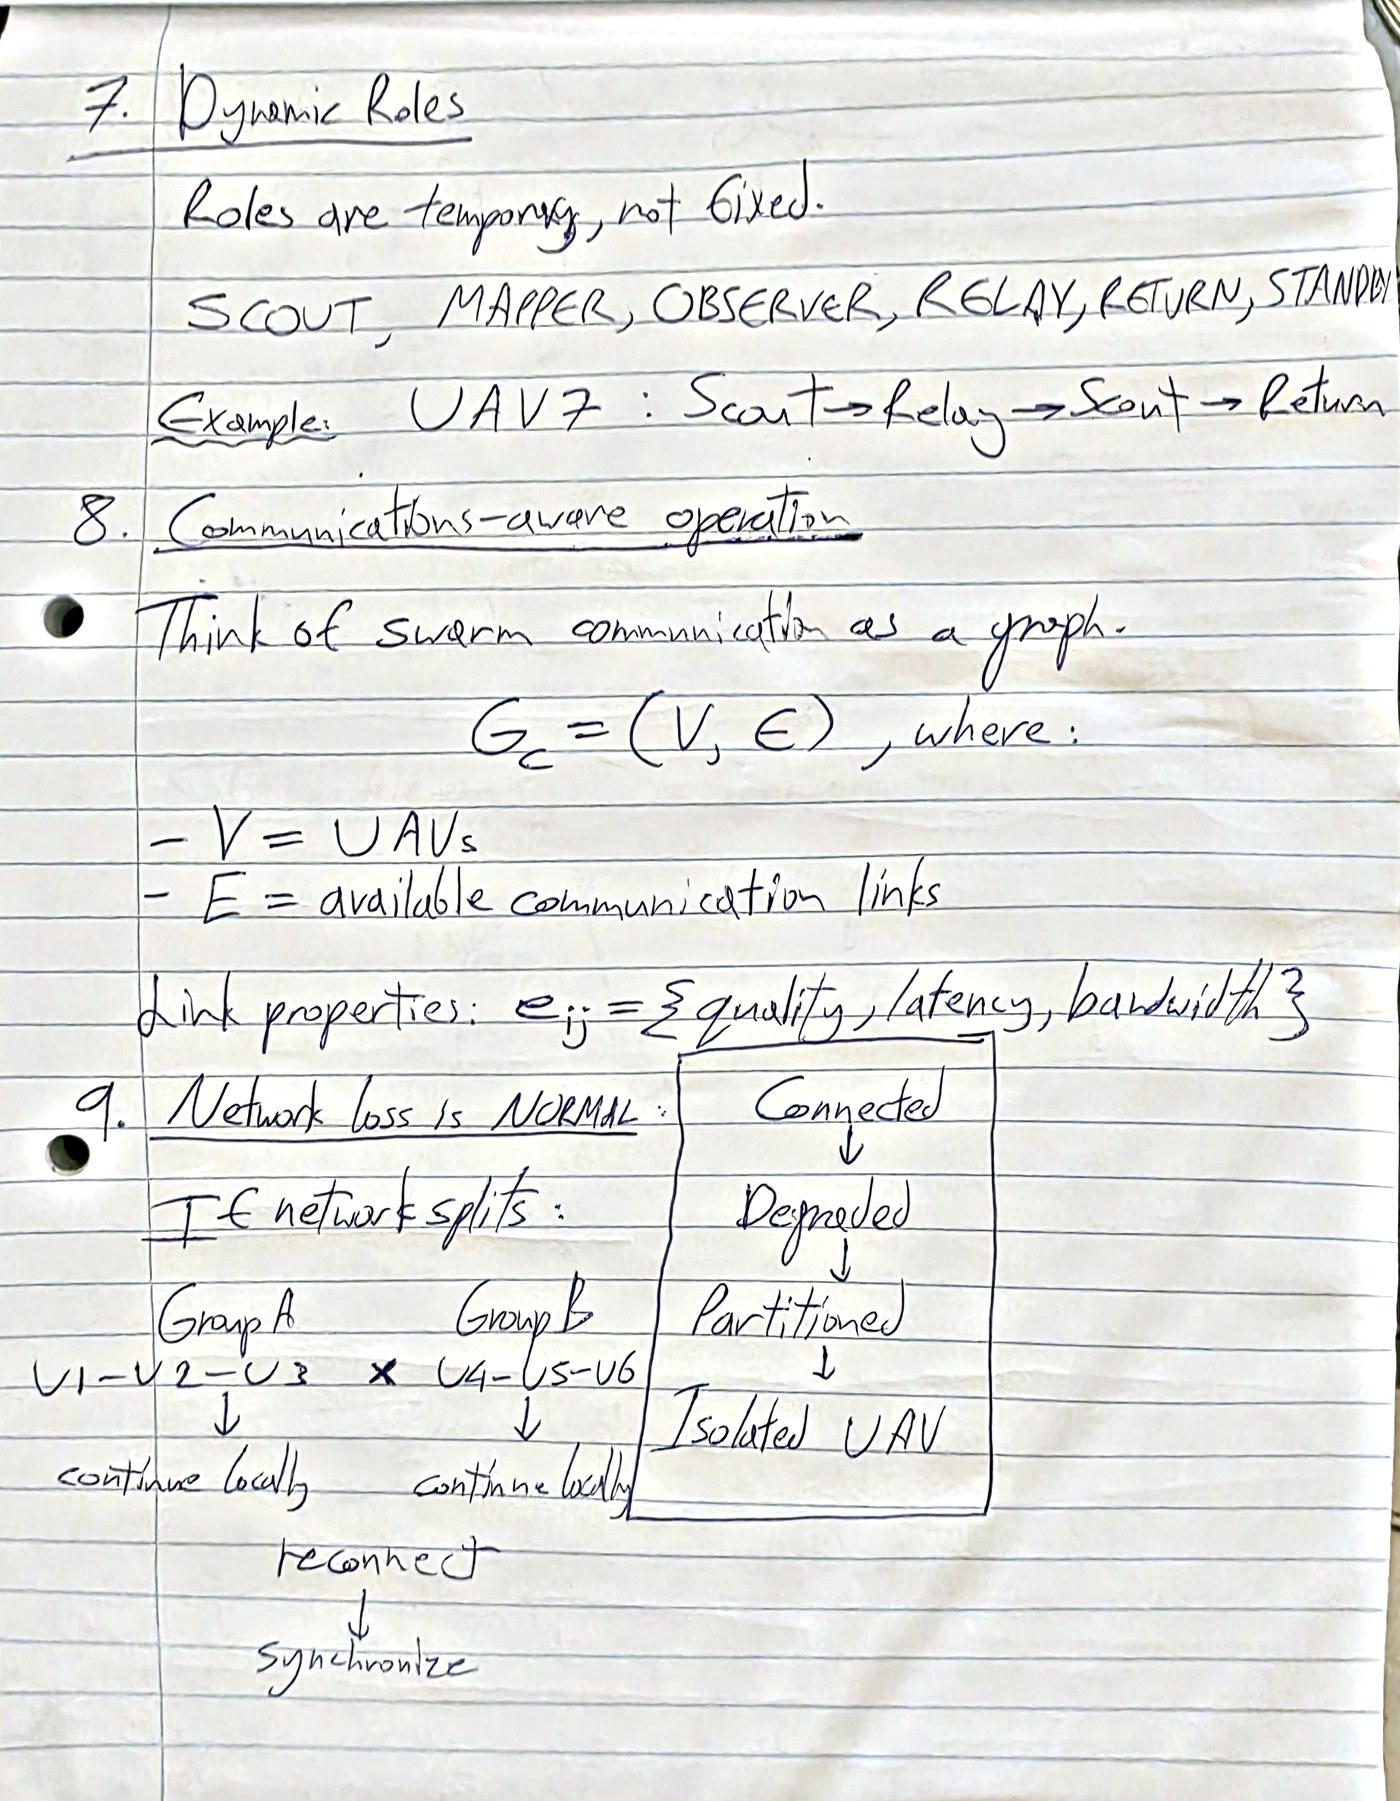
\includegraphics[width=0.31\textwidth]{figures/sketch_comms.jpg}}\hfill
\subfloat[Failure behaviour, utility, safety hierarchy, one-sentence CONOPS.]{%
  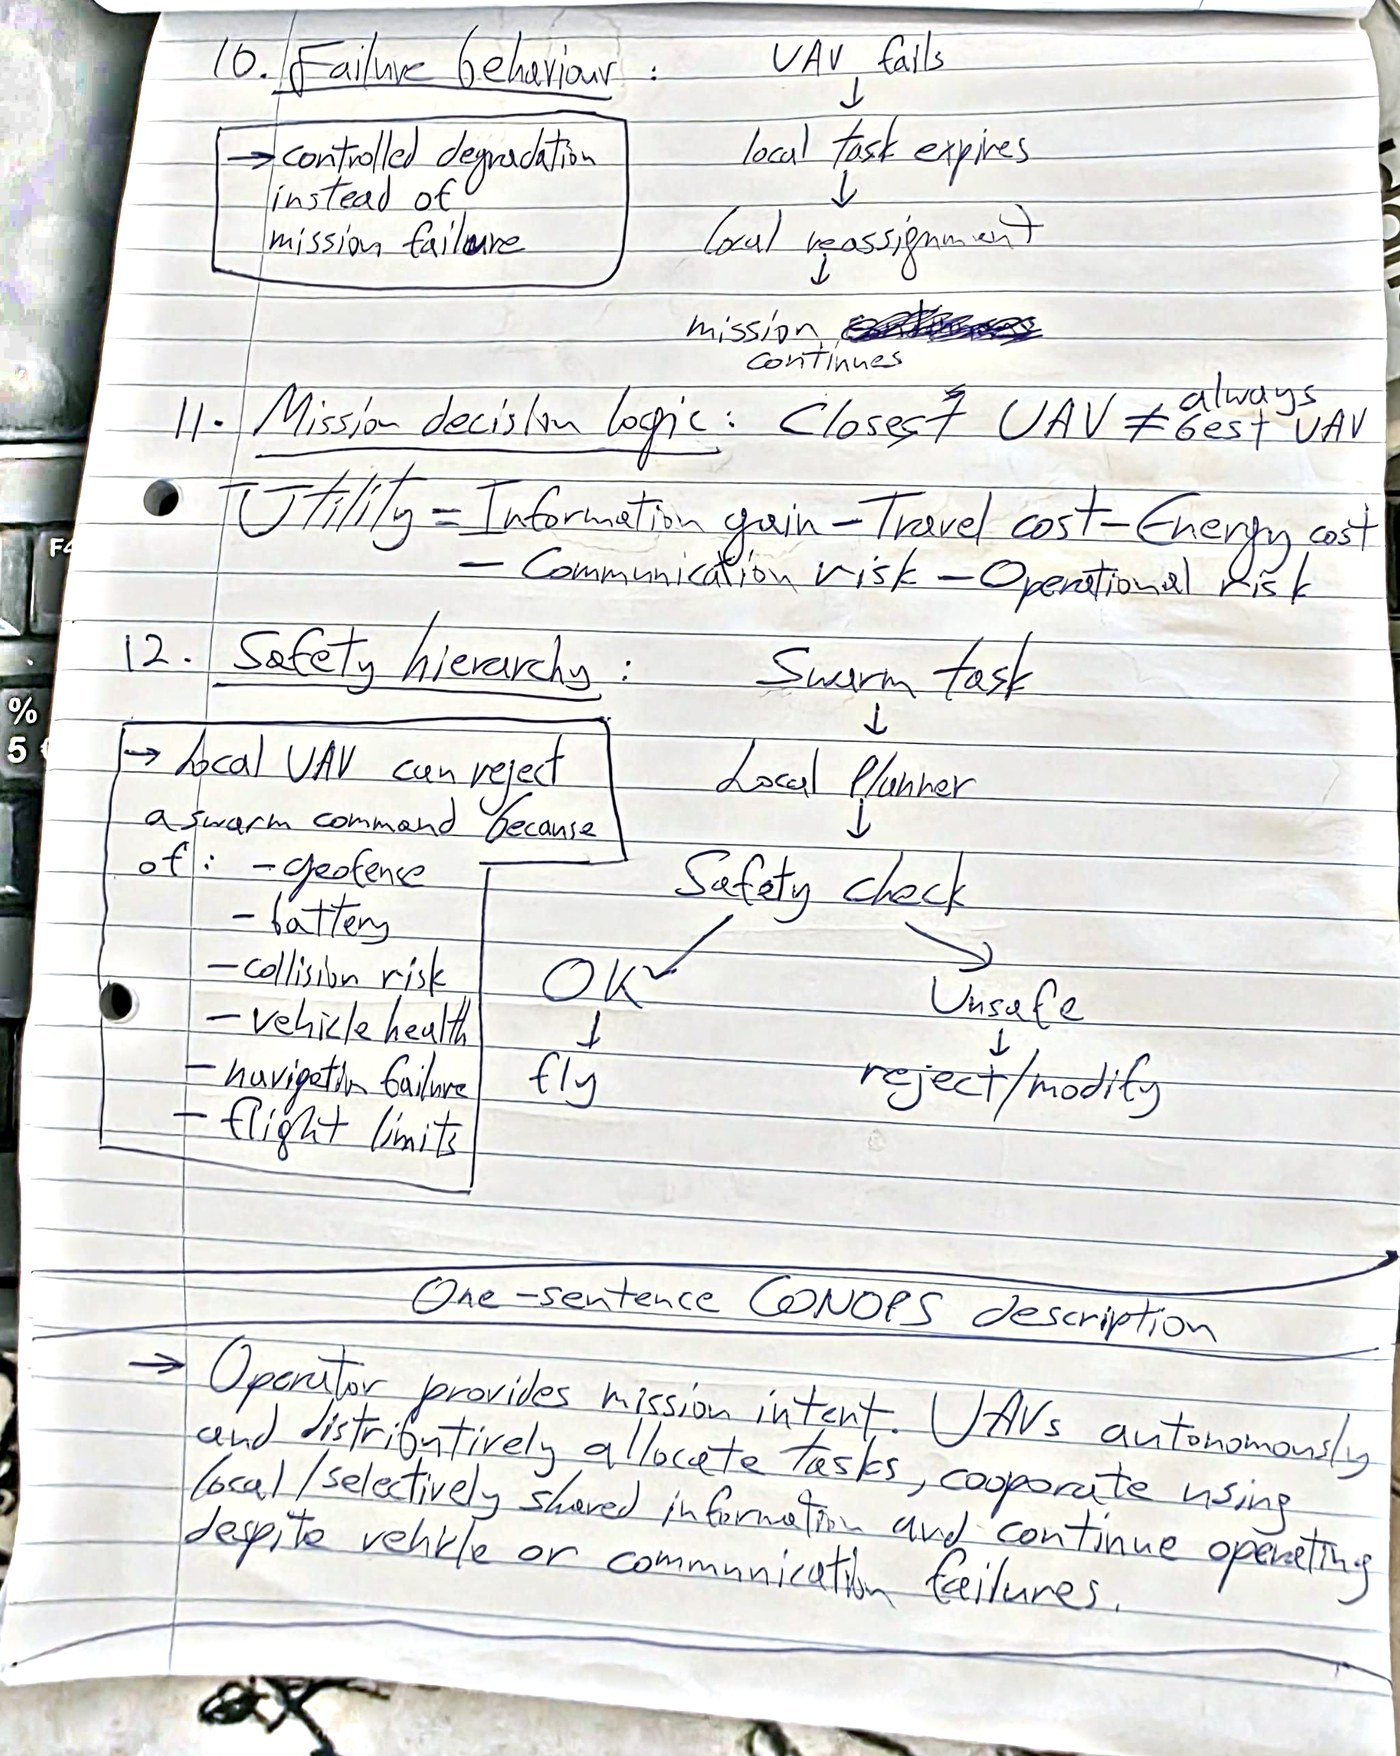
\includegraphics[width=0.31\textwidth]{figures/sketch_failure_safety.jpg}}\hfill
\subfloat[Software architecture: inside every swarm agent.]{%
  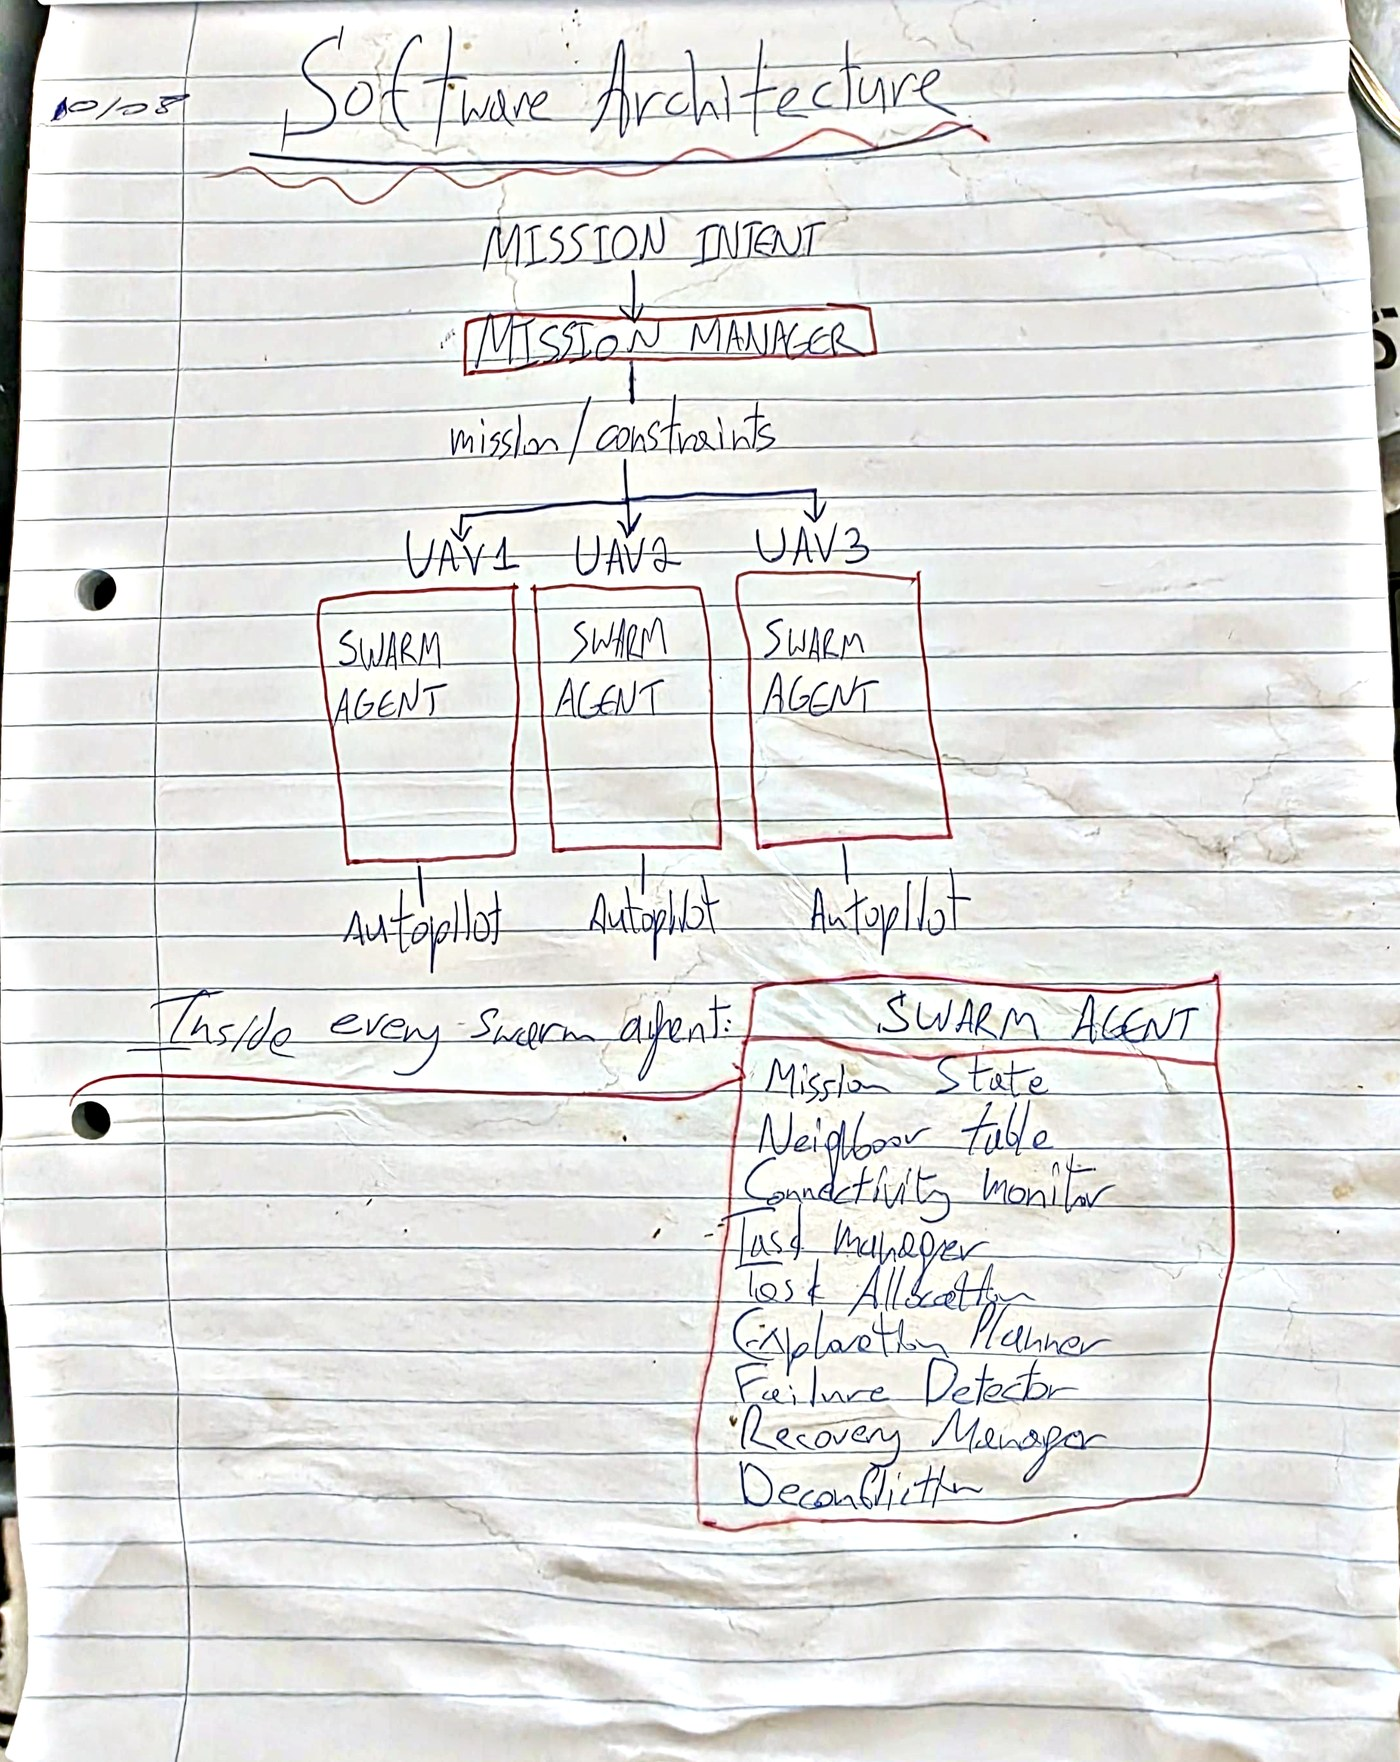
\includegraphics[width=0.31\textwidth]{figures/sketch_architecture.jpg}}
\caption{Original design notebook pages of Team Teleforce.}
\label{fig:sketches}
\end{figure*}

\section{Reproducibility}
\label{app:repro}

Every simulated number in Section~\ref{sec:eval} is regenerated by the
following commands of the \code{eudis-swarm} package; identical seeds give
byte-identical CSV files. The range and lease sweeps are run once per control
mode (option \code{-{}-task-control}). The policy sweep is run once without
a contract and once per policy (option \code{-{}-degradation-policy}).

{\footnotesize
\begin{verbatim}
# range sweep (Fig. 6), once per mode
eudis-swarm-sweep --param communication-range \
  --from 30 --to 130 --steps 11 --seeds 20 \
  --jammer 40,50,15,3,8
# lease sweep (Fig. 7a), once per mode
eudis-swarm-sweep --param lease-timeout \
  --from 0.5 --to 6.0 --steps 12 --seeds 20 \
  --communication-range 50 \
  --failure-time 1000 --jammer 40,50,15,3,8
# degradation policy (Fig. 7b,c)
eudis-swarm-sweep --param communication-range \
  --from 30 --to 90 --steps 7 --seeds 20 \
  --failure-time 1000 --jammer 40,50,15,3,8
# detection floor without jammer (Sec. VI-F)
eudis-swarm-sweep --param communication-range \
  --from 50 --to 130 --steps 9 --seeds 20
# quorum floor (Table IV), split brain (Fig. 5)
eudis-swarm --scenario demo-quorum-floor
eudis-swarm --scenario baseline-quorum-floor
python -m eudis_swarm.task_claim_demo
# fleet/network and layout/fault (Tables V, VI)
eudis-swarm-generalization --seeds 20 --seed-base 1
eudis-swarm-robustness --seeds 20 --seed-base 1
# QAOA benchmark (Table VII), needs [quantum]
python paper/scripts/qaoa_benchmark.py
\end{verbatim}
}

The committed raw CSV files of the fleet and layout studies have SHA-256
digests \code{f23f50f8\ldots{}86e1fe} and \code{582018f1\ldots{}f75576}.
% TODO: decide the licence and public availability of the repository, then
% replace this sentence with a persistent archive link (e.g. a Zenodo DOI).
The source code is available from the authors on request.

\end{document}
